\documentclass[12pt,a4paper,twoside]{report}
\usepackage[utf8x]{inputenc}
%##########################################################################
%Bitte hier die Daten anpassen

\newcommand{\MScBSc}{1} % 0=Bachelorarbeit 1=Projektarbeit 2=Masterarbeit
\newcommand{\Sprache}{1} % 0=Deutsch 1=Englisch 
%Für Bachelor- und Projektarbeiten ist in der Regel Deutsch erwünscht. Bei Masterarbeiten unter Umständen auch Englisch. In jedem Fall gilt: Englische Ausarbeitungen nur nach Absprache mit Professor Seifried!!

% Wenn die Sprache geändert wird muss eventuell zweimal kompiliert werden um eine auftretende Fehlermeldung zu beheben.

\newcommand{\VornameDesStudenten}{Lasse}
\newcommand{\NachnameDesStudenten}{Peters}
\newcommand{\Matrikelnummer}{21486931}
\newcommand{\Studiengang}{Student der Mechatronik} %bitte in diesem Stil lassen!
\newcommand{\Betreuer}{Daniel Duecker, M.Sc.}

\newcommand{\ProfBerkeley}{Prof. Claire J. Tomlin}
\newcommand{\BetreuerBerkeley}{Zachary Sunberg, PhD.}

\newcommand{\NummerDerArbeit}{XXX} % {XXX} durch Nummer der Arbeit ersetzen (diese wird allerdings erst ab ca. 1 Woche vor Abgabe der Arbeit beim Prüfungsamt vom Institut zugeteilt)

%Hier den Titel der Arbeit eintragen
\newcommand{\ThemaDerArbeit}{
		  \Large
          \bf
          \hspace{20mm}Partially Observable\\
          \bf
          \hspace{20mm}Markov Decision Processes\\
          \bf
          \hspace{20mm}for Planning in Uncertain Environments\\}

%##########################################################################

\usepackage{lmodern}
\usepackage{ucs}
\usepackage{xspace}
\usepackage{ifthen}
% Standard Style-Files
\usepackage{amsmath,amssymb,amsthm}
\ifthenelse{\equal{\Sprache}{0}}
    {\usepackage[ngerman]{babel}
    \usepackage[ngerman]{isodate}
    }{}
\ifthenelse{\equal{\Sprache}{1}}
    {\usepackage[latin, ngerman,english]{babel}
    \usepackage[ngerman,english]{isodate}
    }{}
\usepackage{a4}
\usepackage{float} % If we use this package, we can force figures and tables to appear at a certain place. --> use \begin{figure}[H]
\usepackage{flafter} %prevent figures to be displayed before referencing
\usepackage{graphicx}
\usepackage{color}
\usepackage{bm}
\usepackage{import}
\usepackage{subfigure}
\usepackage[autostyle=true,german=quotes]{csquotes}
\usepackage[pdftex,plainpages=false]{hyperref}
\hypersetup{%
    pdfborder = {0 0 0}
} %remove red boxes around section references
\usepackage{bookmark}
\usepackage{fancyhdr}
\usepackage{siunitx}
\usepackage{units}
\usepackage{calc}

% tell TeX that it's infinitely bad to have widows and orphans
\widowpenalty10000
\clubpenalty10000

%%% TIKZ & PGFPLOTS
\usepackage{tikz}
\usepackage{pgfplots}
\pgfplotsset{compat=newest} %globally avoid intereference of ticks and yaxis labels in plots with tikz package

\usetikzlibrary{positioning}
\usepgfplotslibrary{polar}
\usepgfplotslibrary{groupplots}
\usepgfplotslibrary{external}
\usetikzlibrary{pgfplots.groupplots}
\usetikzlibrary{patterns} %for patterns in bar plot
\pgfplotsset{plot coordinates/math parser=false}

%% e.g. pdflatex -synctex=1 -interaction=nonstopmode -shell-escape %.tex  is needed for using tikzexternalize!
\usetikzlibrary{external} %save tikz pictures as pdf and if not changed just use the pdf==>much faster compilation
\tikzexternalize
\makeatletter               % use this to define TiKZ paths for images AND ADD THE BELOW BEFORE INPUTTING EACH CHAPTER
\newcommand{\useexternalfile}[1]{%
    \tikzsetnextfilename{#1-output}%
    \input{\tikzexternal@filenameprefix#1.tikz}}
\makeatother
%%

\usepackage{caption}
\captionsetup{format=hang} % ab zweiter Zeile wird Caption eingerückt



%prevent all capital letter header in table of contents:
\usepackage{etoolbox}
\patchcmd{\tableofcontents}{\MakeUppercase\contentsname}{\contentsname}{}{}
\patchcmd{\tableofcontents}{\MakeUppercase\contentsname}{\contentsname}{}{} %needs to be used twice to work!

% ############################################################################
% Inverse search with xdvi and kile
%
\usepackage{srcltx}
%
% Style-Files
\usepackage{Styles/mum_styles}
% page style
\pagestyle{headings}
% spacing of paragraphs
\setlength{\parskip}{1.5ex}
% don't indent first line of paragraph
\setlength{\parindent}{0pt}
% better spacing of words
\sloppy

% place images where they should be
\setcounter{topnumber}{20}
\setcounter{bottomnumber}{20}
\setcounter{totalnumber}{20}
\renewcommand{\topfraction}{.9999}
\renewcommand{\bottomfraction}{.9999}
\renewcommand{\textfraction}{0}


%##########################################################################
% some special environments
\newtheorem{definition}{Definition}[chapter]
% Call as \begin{definition}[zusatz]  text  \end{definition}
\newtheorem{satz}{Satz}[chapter]
% Call as \begin{satz}[zusatz]  text  \end{satz}

\theoremstyle{definition}
\newtheorem{beispiel}{Beispiel}[chapter]
% Call as \begin{beispiel}[zusatz]  text  \end{beispiel}
\newtheorem{algorithmus}{Algorithmus}[chapter]
% Call as \begin{algorithmus}[zusatz]  text  \end{algorithmus}
\floatstyle{ruled}
\newfloat{algorithm}{thp}{alg}
\floatname{algorithm}{Algorithmus}

%##########################################################################
% define page header
\setlength{\headheight}{15pt}
\pagestyle{fancyplain}
\renewcommand{\chaptermark}[1]{\markboth{\thechapter \hspace{3mm}#1}{}}
\renewcommand{\sectionmark}[1]{\markright{\thesection\ #1}}
\cfoot[\fancyplain{}{}]{\fancyplain{}{}}
\lhead[\fancyplain{}{\small\bf\thepage}]%
{\fancyplain{}{\nouppercase{\small\bf\leftmark}}}
\rhead[\fancyplain{}{\small\bf\rightmark}]%
{\fancyplain{}{\nouppercase{\small\bf\thepage}}}
\renewcommand{\footrulewidth}{0pt}

%##########################################################################
% abbreviations
\newcommand{\tabref}[1]{Tab.~\ref{#1}}

\ifthenelse{\equal{\Sprache}{0}}
    {% Abbildung
    \newcommand{\figref}[1]{Abb.~\ref{#1}}

    % Gleichungs--Referenzen:
    \renewcommand{\eqref}[1]{Gl.~(\ref{#1})}
    }{}
\ifthenelse{\equal{\Sprache}{1}}
{% Abbildung
    \newcommand{\figref}[1]{Fig.~\ref{#1}}

    % Gleichungs--Referenzen:
    \renewcommand{\eqref}[1]{Eq.~(\ref{#1})}
}{}

%###########################################################################

\raggedbottom

\usepackage{sectsty}
\allsectionsfont{\raggedright}

\graphicspath{{Images/}}

\usepackage[numbers]{natbib}
\usepackage{algorithm}
\usepackage[noend]{algpseudocode}
\usepackage{adjustbox}
\makeatletter
\let\OldStatex\Statex
\renewcommand{\Statex}[1][3]{%
  \setlength\@tempdima{\algorithmicindent}%
  \OldStatex\hskip\dimexpr#1\@tempdima\relax}
\makeatother
% setup todo package and make compatible with tikz
\usepackage{todonotes}
% bug fix for `todonotes` vs `tikz` externalize
\usepackage{letltxmacro}
\LetLtxMacro{\oldmissingfigure}{\missingfigure}
\renewcommand{\missingfigure}[2][]{\tikzexternaldisable\oldmissingfigure[{#1}]{#2}\tikzexternalenable}
\LetLtxMacro{\oldtodo}{\todo}
\renewcommand{\todo}[2][]{\tikzexternaldisable\oldtodo[#1]{#2}\tikzexternalenable}

% list of abbreviations
\usepackage{longtable}
\usepackage[acronym, xindy, shortcuts, indexonlyfirst]{glossaries}

% better references
\usepackage[nameinlink, capitalise]{cleveref}
% TODO: maybe overload abbreviations for chapter, figure etc.

\usepackage{lipsum}

% Some useful macros for special formatting. % This doesn't make things
% shorter. It is just a form of typing things to make it easier to change it at
% a later point in time.

% variable names
\newcommand{\vname}[1]{\emph{#1}}
% real numbers
\newcommand{\argmax}{\operatornamewithlimits{argmax}}
\newcommand{\argmin}{\operatornamewithlimits{argmin}}
\newcommand{\reals}{\ensuremath{\mathbb{R}}}
\newcommand{\naturals}{\ensuremath{\mathbb{N}}}
\newcommand{\sspace}{\ensuremath{\mathcal{S}}}
\newcommand{\aspace}{\ensuremath{\mathcal{A}}}
\newcommand{\ospace}{\ensuremath{\mathcal{O}}}
\newcommand{\tdist}{\ensuremath{\mathcal{T}}}
\newcommand{\odist}{\ensuremath{\mathcal{Z}}}
\newcommand{\reward}{\ensuremath{\mathcal{R}}}
\newcommand{\bspace}{\ensuremath{\mathcal{B}}}
\newcommand{\oof}{\ensuremath{\mathcal{O}}}
\newcommand{\qfunction}{$Q$-function\xspace}
\newcommand{\chrond}{\delta}
\newcommand{\pomdpsjl}{\emph{POMDPs.jl}\xspace}
\newcommand{\mode}{\text{mode}\xspace}
\newcommand{\sml}{\ensuremath{s_\text{ml}}}

\newcommand{\ie}{i.e.\ }
\newcommand{\eg}{e.g.\ }

% TODO: example of a rotate figure, maybe helpful for the appendix
%  \begin{figure}[ht]
%    \begin{adjustbox}{addcode={\begin{minipage}{\width}}{\caption{%
%    \todo[inline]{Describe and fix scaling and font}
%        }\end{minipage}},rotate=90,center}
%        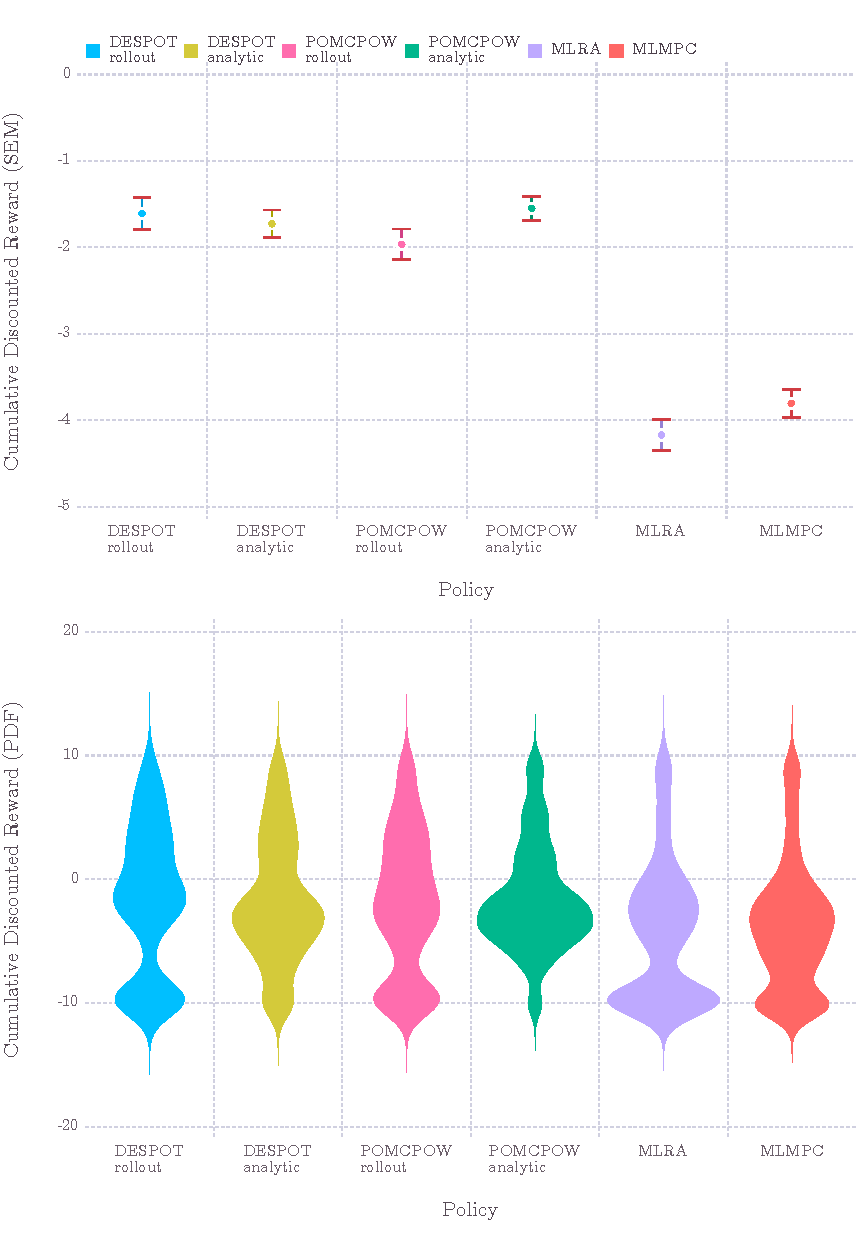
\includegraphics[scale=1]{roomba_plots/lp_value_eval_plot.pdf}
%    \end{adjustbox}
%  \end{figure}

% abbreviations:
\newacronym[plural=MDPs, longplural=Markov Decision Processes]{mdp}{MDP}{Markov Decision Process}
\newacronym[plural=POMDPs, longplural=Partially Observable Markov Decision Processes]{pomdp}{POMDP}{Partially Observable Markov Decision Process}
\newacronym[plural=MOMDPs, longplural=Mixed Observability Markov Decision Processes]{momdp}{MOMDP}{Mixed Observability Markov Decision Process}
\newacronym{mcts}{MCTS}{Monte-Carlo Tree Search}
\newacronym{pomcp}{POMCP}{Partially Observable Monte-Carlo Planning}
\newacronym{pomcpow}{POMCPOW}{Partially Observable Monte-Carlo Planning with Observation Widening}
\newacronym{despot}{DESPOT}{Determinized Sparse Partially Observable Tree}
\newacronym{dpw}{DPW}{Double Progressive Widening}
\newacronym{uct}{UCT}{Upper Confidence Bound for Trees}
\newacronym{hri}{HRI}{Human Robot Interaction}
\newacronym{mlmpc}{MLMPC}{Most Likely Model Predictive Control}
\newacronym{mpc}{MPC}{Model Predictive Control}
\newacronym{mlra}{MLRA}{Most Likely Reflex Agent}
\newacronym{sem}{SEM}{Standard Error of the Mean}
\newacronym{pdf}{PDF}{Probability Density Function}
\newacronym{psrp}{PSRP}{Probabilistically Safe Robot Planning}
\makeglossaries


\begin{document}
% with this command the path for tikZ pcitures always assumes to be in
% Images/... change this if needed, e.g. at the beginning of each chapter
\tikzsetexternalprefix{Images/}

%###########################################################################
%
%   Titelseite
%
%###########################################################################
\begin{titlepage}

\hspace{20mm}\begin{minipage}{0.3\linewidth}
		 \ifthenelse{\equal{\MScBSc}{0}}
			{\ifthenelse{\equal{\Sprache}{0}}
				{\textbf{Bachelorarbeit}\\
				\large{BSC-\NummerDerArbeit}}{}
			\ifthenelse{\equal{\Sprache}{1}}
			{\textbf{Bachelor's Thesis}\\
				\large{BSC-\NummerDerArbeit}}{}
			}{}
		\ifthenelse{\equal{\MScBSc}{1}}
			{\ifthenelse{\equal{\Sprache}{0}}
				{\textbf{Projektarbeit}\\
				\large{PRO-\NummerDerArbeit}}{}
				\ifthenelse{\equal{\Sprache}{1}}
				{\textbf{Project Thesis}\\
				\large{PRO-\NummerDerArbeit}}{}
			}{}
		\ifthenelse{\equal{\MScBSc}{2}}
			{\ifthenelse{\equal{\Sprache}{0}}
				{\textbf{Masterarbeit}\\
				\large{MSC-\NummerDerArbeit}}{}
				\ifthenelse{\equal{\Sprache}{1}}
				{\textbf{Master's Thesis}\\
				\large{MSC-\NummerDerArbeit}}{}
			}{}

	 	 
\end{minipage}\hfill
\begin{minipage}{0.3\linewidth}
	
\includegraphics[height=45pt]{Styles/mum_logo.pdf}
\end{minipage}
\vspace{8mm}
\begin{center}
	\vspace{20mm}
    {\ThemaDerArbeit}
	\vspace{10mm}
	\ifthenelse{\equal{\Sprache}{0}}
	{\hspace{20mm}{\normalsize von}\large\\
	}{}
	\ifthenelse{\equal{\Sprache}{1}}
	{\hspace{20mm}{\normalsize by}\large\\
	}{}
	\hspace{20mm}{\large \VornameDesStudenten \ \NachnameDesStudenten}\\
	\vspace{30mm}
	\normalsize
	\ifthenelse{\equal{\Sprache}{0}}
	{	\hspace{20mm}\begin{tabular}{rl}
			Betreuer: & Prof. Dr.-Ing. R. Seifried \\
			& \Betreuer
		\end{tabular}\\
			\vfill
			\large
			\hspace{20mm}Technische Universität Hamburg-Harburg (TUHH) \\
			\hspace{20mm}Institut für Mechanik und Meerestechnik\\
			\hspace{20mm}Prof.\ Dr.-Ing.\ R.\ Seifried
		}{}
	\ifthenelse{\equal{\Sprache}{1}}
    {
     \hspace{20mm}\begin{tabular}{cc}
            \textbf{Supervisors at TUHH} & \textbf{Supervisors at UC Berkeley}\\
            Prof. Dr.-Ing. Robert Seifried & \ProfBerkeley\\
            \Betreuer & \BetreuerBerkeley
        \end{tabular}\\
            \vfill
            \large
            \hspace{20mm}Hamburg University of Technology \\
            \hspace{20mm}Institute of Mechanics and Ocean Engineering\\
            \hspace{20mm}Prof.\ Dr.-Ing.\ R.\ Seifried
        }{}

\end{center}
\vspace{1cm}
\begin{center}
	\ifthenelse{\equal{\Sprache}{0}}
	{		{\large \hspace{20mm} Hamburg,
%			\month=\the\month
%			\makeatletter
%			\month@ngerman
%			\makeatother~\the\year
			\printdayoff \today \printdayon}}{}
	\ifthenelse{\equal{\Sprache}{1}}
	{	{\large \hspace{20mm} Hamburg, 
			\printdayoff \today \printdayon
	}}{}

\end{center}
\end{titlepage}

\clearpage
\thispagestyle{empty}
\cleardoublepage

% Start content on the right hand side.
\thispagestyle{empty}\cleardoublepage
% margins for double sided printing
\evensidemargin=2pt
\oddsidemargin=40pt

% proper line spacing
\renewcommand{\baselinestretch}{1}\normalsize
\pagenumbering{roman}
% Table of contents
\tableofcontents
\cleardoublepage

\pagenumbering{arabic}
\printglossary[type=\acronymtype,title=List of Abbreviations]
% TODO: one could also add nomenclature maybe
\chapter{Introduction}\label{chap:introduction}

\todo[inline]{General, broad introduction to Planning in Uncertain Environments
in the real world featuring some state of the art work.}.
\begin{itemize}
  \item why does considering uncertainty matter
  \item very brief introduction to POMDP which can be mainly copied from the project proposal
  \item why is it challenging to do it like this, why do people avoid this:
        point to planning on expectation and making certain assumptions on the structure to
        make the problem simpler or neglecting the fact that
        in the future the agent get additional information
  \item point to literature of examples for this kind of problems
  \item very brief summary what this work is going to show / what is the point
        of this work (just a very short paragraph). Details can be mentioned in the
        "motivation" section. (this can be refined at the end)
\end{itemize}

\section{Motivation}

\todo[inline]{Motivate this work. Maybe this does not need to be a separate subsection.}

\begin{itemize}
  \item this work seeks to explore the use of POMDPs for planning in uncertain environments
  \item looking at two popular problems (localization and motion planning)
  where partial observability is usually neglected or treated with significant
  simplifications, what is the performance gain that can be achieved.
\end{itemize}

\section{Chapter Outline}

\todo[inline]{write, when structure has converged}

\todo[inline]{Project proposal. Placed here as a template}
The \textit{partially observable Markov decision process} (POMDP) provides
a principled general framework for planning in partially observable stochastic
environments. In contrast to their well known fully observable counter part,
the \textit{Markov Decision Process} (MDP), in a POMDP the agent can not access
state information directly. Instead, the agent is presented with observations
as stochastic emissions of the true state of the world. Therefore, solving
a POMDP requires the planner to reason about a distribution over possible
futures with uncertainty in both the transition and observation model. This
makes solving a POMDP a significantly more challenging problem than solving the
corresponding fully observable MDP.\\

A POMDP is a PSPACE-complete problem and thus optimal solutions to problems of
this class can not be found in polynomial time. Therefore, in robotics
applications, characterized by limited compute and real time constraints, POMDP
solution methods are traditionally avoided. Instead, simplifications are made
that neglect the partial observability or make other assumptions about the
problem structure.\\

This project aims to explore how despite these challenges the POMDP
framework can be used to compute robust policies for a robot to optimally
interact with an uncertain environment. For this purpose, uncertainty in
two different subsets of the state space are considered:\\
\textit{External States,}  states of the environment. (e.g. position of the
robot).\\
\textit{Internal States,} latent \textit{model parameters} of the
environment (e.g. intentions of other agents).\\

The use of POMDP solution methods for planning in the face of uncertainty in
each of these domains will be examined. External state uncertainty will be
studied in a simulated environment at the example of simultaneous localization
and planning. Internal state uncertainty will be studied at the example of
human robot interaction.\\
In order to address the issue of limited compute in the context of robotics
applications, this project will investigate how meta reasoning can be employed to
dynamically switch models during on-line planning in an effort to account for
the trade-off between accuracy and computational complexity when reasoning about
future environment states.

\chapter{Fundamentals}\label{chap:fundamentals}

This work showcases the use of \acp{pomdp} to model and solve decision making
problems in robotics with inherent uncertainty. In order to provide a baseline
for further discussions of specific application domains
(\cref{chap:localization-and-planning,chap:hri}) we first
introduce some of the throughout this work. It should be noted that in the
interest of conciseness we focus this theoretical introduction on only the main
tools use. Fundamental concepts of statistical inference and tools like
\textit{Monte Carlo Integration} are assumed to be known. For a thorough
discussion of these underlying concept the reader may refer to
\cite{kochenderfer2015decision, bertsekas2005dynamic, thrun2005probabilistic}.

In the following, we first introduce the theoretical framework of \acp{pomdp}
used for sequential decision making under uncertainty
(\cref{sec:sequential-decision-making}). This section discusses modelling
assumptions, structure of solutions as well as theoretical properties of
\acp{pomdp}. Thereafter, \cref{sec:online-pomdp-solvers} describes two
state-of-the-art online solution methods for problems of this domain.

\section{Sequential Decision Making Problems Under Uncertainty}\label{sec:sequential-decision-making}

The \acf{pomdp} is a principled mathematical formalism capable of representing
a broad range of sequential decision making problems under uncertainty. As the
name suggests, this framework is a generalization of the more popular \ac{mdp}
to the partially observable case. Thus, before proceeding with the full
complexity of a \ac{pomdp} let us first examine it's fully observable version.

\subsection{Markov Decision Process (MDP)}\label{sec:mdp}

\acfp{mdp} are sequential decision making problems in which an agent takes
\vname{actions} $a$ that affect the \vname{state} $s$ of the environment and
receives \vname{rewards} $r$ based the state-transition and the action taken
\cite{kochenderfer2015decision, bertsekas2005dynamic}. The state evolves
according to a stochastic transition model $\tdist$ that and obeys the
Markov property. That is, future states are independent of past states given
the current state and action. By this means, \acp{mdp} allow to model outcome
uncertainty. As common in literature, we denote quantities at time time $t$
with an according subscript. When examining only a single step in a context
where time does not explicitly matter, we may also refer to states before and
after the transition as $s$ and $s'$ rather than $s_t$ and $s_{t+1}$.

Formally, an \ac{mdp} is fully characterized by the following quantities:

\begin{description}
  \item[State Space $\sspace$.] The set of all possible states.
  \item[Action Space $\aspace$.] The set of all possible actions.
  \item[Transition Model $\tdist$.] A model to represent the likelihood of
    each transition. This model provides $\tdist(s' \mid s, a)$, the
    probability of state $s'$ given that previously the environment was in
    state $s$ and the agent took action $a$.
  \item[Reward Function $\reward: \sspace \times \aspace \times
    \sspace \to \reals$.] A deterministic mapping that assigns
    a real-valued reward $r$ to each transition $(s, a, s')$ with finite transition
    probability, $\tdist(s' \mid s, a) > 0$.
  \item[Discount Factor $\gamma$.] A scalar that governs how rewards
    are discounted in the future.
\end{description}

The objective of the agent in the \ac{mdp} is to maximize the expected
cumulative rewards. Formally, this translates to finding a \vname{policy} $\pi:
\sspace \to \aspace$, that maps each encountered $s$ to an action $a
= \pi(s)$, such that following this policy maximizes the objective,

\begin{equation} \label{eq:objective}
    J(\pi) = E\left[\sum_{t=0}^\infty \gamma^t \reward(s_t, \pi(s_t), s_{t+1})\right] \text{.}
\end{equation}

An optimal solution to an \ac{mdp} can always be formulated as a deterministic
Markov policy, even though the reward that a policy achieves may be randomized
through $\tdist$. Consequently, there always exists a maximizer $\pi^*$ of
\cref{eq:objective}, where $\pi^*$ assigns a single action to every state.
Also, since the state obeys the Markov property, no additional information
beyond the current state at every time is necessary to maximize $J$
\cite{altmann1999constrained}.

\todo[inline]{Maybe this is a good point to also quickly introduce value functions?}

\subsection{Partially Observable MDP (POMDP)}\label{sec:pomdp}

A \acf{pomdp} is an \ac{mdp} where the agent cannot directly observe the state,
but instead at every time step $t$ receives an \vname{observation} $o_t$,
emission of the latent state $s_t$ and action $a_t$. By this means,
a \ac{pomdp} is able to encode state uncertainty in addition to the outcome
uncertainty present in the underlying \ac{mdp}.

Having introduced the properties of an \ac{mdp} in the previous section,
a generalization of this formalism to the partially observable case is obtained
by augmenting the 5-tuple $(\sspace, \aspace, \tdist, \reward,
\gamma)$ describing the underlying \ac{mdp} with the following quantities:

\begin{description}
  \item[Observation Space $\ospace$.] The set of all possible observations.
  \item[Observation Model $\odist$.] A model to represent the likelihood
    of each observation $o$ given the current state of the environment and the
    action taken at that time. Formally, this model provides the
    conditional probability $\odist(o \mid s, a)$ for each $(o, s, a) \in
    (\ospace \times \sspace \times \aspace)$.
\end{description}

The dynamic decision network representing the information structure for
a finite time horizon \ac{pomdp} is depicted in \cref{fig:pomdp}. As evident
from this figure, the decision of the agent at time $t$ is informed by the
sequence of all previous actions and observations as well as some prior
knowledge, $b_0$. In contrast to the fully observable case where the policy is
only a function of quantities at the current time, the policy in a \ac{pomdp}
maps each possible \vname{history}, ${h_t = (b_0, a_0, o_1, a_1, \dots,
a_{t-1}, o_t)}$ to an action, $a_t$.

\begin{figure}[htpb]
  \centering
  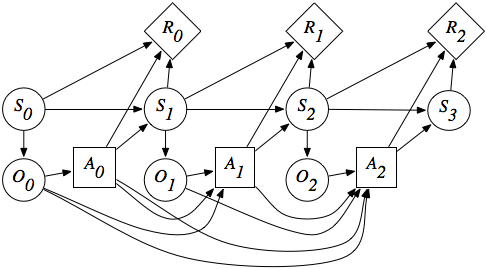
\includegraphics[width=.7\textwidth]{pomdp-dynamic-decision-network.png}
  \caption{The POMDP as a dynamic decision network. \todo[inline]{Replace with
  vector graphics and add initial information $b0$}}
  \label{fig:pomdp}
\end{figure}

In cases where this history can be compressed to a probability for every state
at time $t$, we will refer to this distribution as the \vname{belief},
$b_t(s)$. This belief is a sufficient statistic for optimal decision making.
Consequently, there exists a policy $\pi^*(b_t)$ only dependent on the belief
at the current time step, such that choosing ${a_t=\pi^*(b_t)}$ maximizes
\cref{eq:objective} subject to the constraints on the information pattern
imposed by the \ac{pomdp}, \cite{kaelbling1998planning,
kochenderfer2015decision}. Loosely speaking, $b_t$ preserves all relevant
information contained in the action-observation-history, $h_t$ necessary to
compute the optimal action. The belief is maintained by recursively performing
a Bayesian update,
\begin{equation} \label{eqn:update}
    b'(s') = \frac{\int_{s\in\sspace} \odist(o \mid s, a, s') \tdist(s' \mid s, a) b(s) \, ds}
    {\int_{s'\in\sspace} \int_{s\in\sspace} \odist(o \mid s, a, s') \tdist(s' \mid s, a) b(s) \, ds \, ds'} \text{.}
\end{equation}
with incoming observations, $o$. In the case of a discrete state space,
$\sspace$ integrals a to be replaced with sums. In cases where this update rule
is too complex to be evaluated analytically, Monte Carlo integration may be
used for approximate inference \cite{kochenderfer2015decision,
thrun2005probabilistic}.

Solutions to a \ac{pomdp} are Markov policies on belief states. That is, the
optimal policy $\pi^*(b(s)): \bspace \to \aspace$ selects action ${a =
\pi(b(s))}$ for each belief in the \vname{belief space}, $\bspace$ under the
objective of maximizing \cref{eq:objective}. Alternatively, when thinking of
this procedure in terms of action-observation-histories, the policy may be
envisioned as a conditional plan reasoning over the optimal action to take for
every possible sequence of actions and observations starting from the root
belief, $b_0$. This perspective reveals that the search space of possible
policies rapidly grows with increasing size of $\aspace$ and $\ospace$. In
fact, it has been shown that even in the case of finite-horizon problems
\acp{pomdp} remain PSPACE-complete. Hence, it is reasonable to assume to that
no efficient general algorithm for solving large problems of this class can be
found \cite{papadimitriou1987complexity}. However, recent research has made
significant progress on approximate solution methods, some of which we will use
in this work \cite{silver2010pomcp, somani2013despot, sunberg2018online}.

\section{Online POMDP Solvers}\label{sec:online-pomdp-solvers}

Once a problem has been formalized as a \ac{pomdp}, a wide range of solution
methods can be applied to solve it. On an abstract level, there exist two classes
of solution techniques:

\emph{Offline} methods perform most of the computation prior to execution. That
is, a policy for the entire belief space is computed a priori. At execution
time, actions are selected according to the assignment computed offline.

\emph{Online} methods compute the optimal policy at execution time by planning
from the current belief state. Solution techniques of this kind potentially
leads to redundant computation and more compute per decision step at runtime.
However, in practice they allow to solve much larger \acp{pomdp} since the
reachable belief states are typically a small subset of the full belief space.
By exploiting this local structure online methods allow to compute solutions to
large problems that may be intractable for offline approaches
\cite{kochenderfer2015decision, silver2010pomcp, somani2013despot,
kurniawati2016online}.

In practice, due to the complexity of \acp{pomdp}, even for seemingly simple
problems finding the exact solution is computationally intensive. However,
recent research has put forth online solvers that provide good approximations
to a wide range of problems. This work makes use of two of the most elaborate
state of the art online \ac{pomdp} solvers -- \ac{despot} and \ac{pomcpow}. We
choose these methods since they show superior performance in a wide range of
benchmark problems and outperform other approximate solutions especially for
large \acp{pomdp} \cite{somani2013despot, sunberg2018online}.

In the following subsections we introduce \ac{despot} and \ac{pomcpow} in
greater detail and discuss their theoretical properties.

\subsection{DESPOT}

\begin{algorithm}[htpb]
  \caption{DESPOT \cite{somani2013despot}.}\label{alg:despot}
  \begin{algorithmic}[1]
    \Procedure{Plan}{$b_0$}
      \State $\ell \gets \Call{BuildDespot}{b_0}$
      \State $a^* \gets \max_{a \in \aspace}{\ell(b_0, a)}$
      \If{$L_0(b_0) > \ell(b, a^*)$}
        \State $a^* \gets \pi_0(b_0)$
      \EndIf
      \State \textbf{return} $a^*$
    \EndProcedure\vspace{10pt}

    \Procedure{BuildDespot}{$b_0$}
      \State $\Phib_{b0} \gets K \text{ scenarios sampled from } b_0$
      \State $\mathcal{D} \gets \text{new DESPOT with a single node $b_0$ as the root}$
      \State Initialize $U(b_0), L_0(b_0), \mu(b_0),$ and $\ell(b_0)$ \Comment{TODO: Explain}
      \State $\epsilon(b_0) \gets \mu(b_0) - \ell(b_0)$
      \While{$\epsilon(b_0) > \epsilon_0$ and total running $< T_{\text{max}}$}
        \State $b \gets \Call{Explore}{\mathcal{D}, b}$
        \State $\Call{Backup}{\mathcal{D}, b}$
        \State $\epsilon(b_0) \gets \mu(b_0) - \ell(b_0)$ \Comment{TODO: Think about this}
      \EndWhile
      \State \textbf{return} $\ell$
    \EndProcedure\vspace{10pt}

    \Procedure{Explore}{$\mathcal{D}, b$}
      \While{$\Delta(b) \leq D, E(b) > 0, \text{ and } \Call{Prune}{\mathcal{D}, b} = \text{FALSE}$}
        \If{$b$ is a leaf node in $\mathcal{D}$}
          \State Expand $b$ one level deeper.
          \Statex[3] Insert each new child $b'$ of $b$ into $\mathcal{D}$,
          \Statex[3] and initialize $U(b'), L_0(b'), \mu{(b')}$, and $\ell(b')$.
        \EndIf
        \State $a^* \gets \argmax_{a \in \aspace}{\mu(b, a)}$
        \State $o^* \gets \argmax_{o \in \ospace_{b, a^*}}{E(\tau(b, a^*, z))}$\Comment{Think about this}
        \State $b \gets \tau(b, a^*, z^*)$
      \EndWhile
      \If{$\Delta(b) > D$}
        \State $\Call{MakeDefault}{b}$
      \EndIf
      \State \textbf{return} $b$
    \EndProcedure\vspace{10pt}
  \end{algorithmic}
  \todo[inline]{Figure out how to space this properly.}
  \todo[inline]{Figure out multi column or multi page solution.}
\end{algorithm}

\begin{algorithm}[htpb]
  \begin{algorithmic}[1]
      \Procedure{Prune}{$\mathcal{D}, b$}
        \State \textsc{Blocked} $\gets$ FALSE
        \For{each node $n$ on the path from $b$ to the root of $\mathcal{D}$}
          \If{$n$ is blocked by any ancestor node in $D$}
            \State $\Call{MakeDefault}{n}$
            \State $\Call{Backup}{\mathcal{D}, n}$
            \State \textsc{Blocked} $\gets$ TRUE
          \Else
            \State \textbf{break}
          \EndIf
        \EndFor
        \State \textbf{return} \textsc{Blocked}
      \EndProcedure\vspace{10pt}

      \Procedure{MakeDefault}{$b$}
        \State $U(b) \gets L_0(b)$
        \State $\mu(b) \gets l_0(b)$
        \State $\ell(b) \gets \ell_0(b)$
      \EndProcedure\vspace{10pt}

      \Procedure{Backup}{$\mathcal{D}, b$}
        \For{each node $n$ on the path form $b$ to the root of $D$}
          \State Perform backup on $\mu(x), l(x)$, and $U(x)$.
        \EndFor
      \EndProcedure\vspace{10pt}
  \end{algorithmic}
\end{algorithm}

\todo[inline]{write:}
\begin{itemize}
  \item formal, high-level idea of a DESPOT (idea of scenarios etc.)
  \item the search algorithm on a DESPOT with bounds
  \item explain the difference to POMCPOW (or Monte Carlo methods in general)
  \item point to literature for convergence guarantees
\end{itemize}

\missingfigure{DESPOT tree visualization}

\subsection{POMCPOW}

\acf{pomcpow} is an approximate online \ac{pomdp} solver that combines the idea
of \ac{mcts} -- as utilized in \ac{pomcp} \cite{silver2010pomcp} -- with the
idea of \ac{dpw} \cite{sunberg2018online}.

Before we discuss the algorithmic procedure of \ac{pomcpow} we briefly review
the general idea of \ac{mcts}. This section is thought to be a concise recap of
the fundamental concept and seeks to provide a baseline for understanding how
this technique is adopted in the context of \ac{pomcpow}. A thorough discussion
of \ac{mcts} goes beyond the scope of this work. For a detailed survey of
a wide range of \ac{mcts} algorithms, the reader may refer to
\cite{browne2012survey}.

\subsubsection{Monte-Carlo Tree Search}
A theoretically valid solution method for sequential decision making problems
is the construction of the entire policy tree. This tree consists of alternating
layers of states and actions, enumerating all possible future trajectories.
Given this object, extracting the optimal strategy from is trivial. However,
for problems relevant in practice the curse of dimensionality makes simulating
all possible futures intractable.

\acf{mcts} is a method that breaks the curse of dimensionality by utilizing
Monte-Carlo simulations to incrementally construct only important parts of the
policy tree in an asymmetric fashion. As the policy is constructed, the samples
are used to approximate the \vname{state-action value function}, $Q(s, a)$,
also referred to as the \vname{\qfunction}. The approximate \qfunction is used
to focus further exploration of promising parts of the tree, allowing the
algorithm to approximate the optimal policy without attempting the intractable
task of constructing the entire policy tree. This behavior is achieved by
invoking a suitable \emph{tree policy} that balances exploration and
exploitation, the trade-off between looking at new parts of the state-action
space (widening the tree) and further exploring promising trajectories
(deepening the tree). One reason for the popularity of this method is that
it only requires access to a \vname{generative model}, $G$, used to sample new states
given a state-action a pair. That is, no explicit model of the state dynamics is
required, as long as a black box simulator of the environment is available.

To date, \ac{mcts} has been applied to a wide range of problems
\cite{browne2012survey}. While research has put forth many variants of this
algorithm, conceptually they all share the idea of iteratively running
Monte-Carlo simulations until a terminal condition is reached. This terminal
condition may be derived from a convergence criterion, a fixed number of
iterations or a limited computational budget. One iteration of the general
\ac{mcts} algorithm is visualized in \cref{fig:mcts-general}. Each cycle
comprises four steps:

\begin{description}
  \item[Search] The tree policy is invoked to traverse the policy tree
    constructed up to this point. That is, at each state node the tree policy
    selects an action based on the current \qfunction approximation. Once an
    action has been chosen, the next state is selected by sampling from the
    $G$. This search procedure is repeated in an effort to reach
    the most urgent leaf node of the policy tree.
  \item[Expansion] Once an action node is reached that does not have any
    children, a new node is appended to the policy tree by sampling a state
    from $G$ and adding the corresponding actions.
  \item[Rollout] Starting from the newly added node, a reward trajectory is
    simulated by selecting actions according to a \emph{rollout policy}. This
    rollout policy may be as trivial as randomly selecting actions until
    a terminal state is reached or the future cumulative reward becomes
    negligible due to the compounding discount factor. Alternatively, domain
    specific knowledge may be utilized to design a more structured rollout
    strategy. The rollout yields a value estimate for the newly added leaf node.
  \item[Backpropagation] The value estimate obtained from the rollout
    simulation is passed back up the tree to update the \qfunction estimate on
    the path to the root node.
\end{description}

An important factor for the success of of this algorithm is the choice of the
tree policy as this policy must focus the expansion to the relevant part of the
tree. A widely used tree policy is the \ac{uct}. This policy is a greedy policy
with respect to the \vname{upper confidence bound},
\begin{equation}
\label{eqn:ucb} \emph{UCB}(s,a) = Q(s,a) + c \sqrt{\frac{\log N(s)}{N(s,a)}}.
\end{equation}

Here, $N(s, a)$ is the number of times the action node (child) has been
visited, $N(s) = \sum_{a \in \aspace}{N(s, a)}$ is the number of times the
corresponding state node (parent) has been visited, and $c$ is a problem
specific parameter to balance the exploration/exploitation trade-off.
Intuitively, the first term encourages the algorithm to select actions that in
the past showed promising future reward trajectories while the second term
urges the tree policy to expand nodes that have not been sufficiently explored.
For a thorough discussion of convergence properties as well as guidance for the
tuning of $c$, the reader may refer to \cite{kocsis2006bandit, browne2012survey}.

\begin{figure}[htpb]
  \centering
  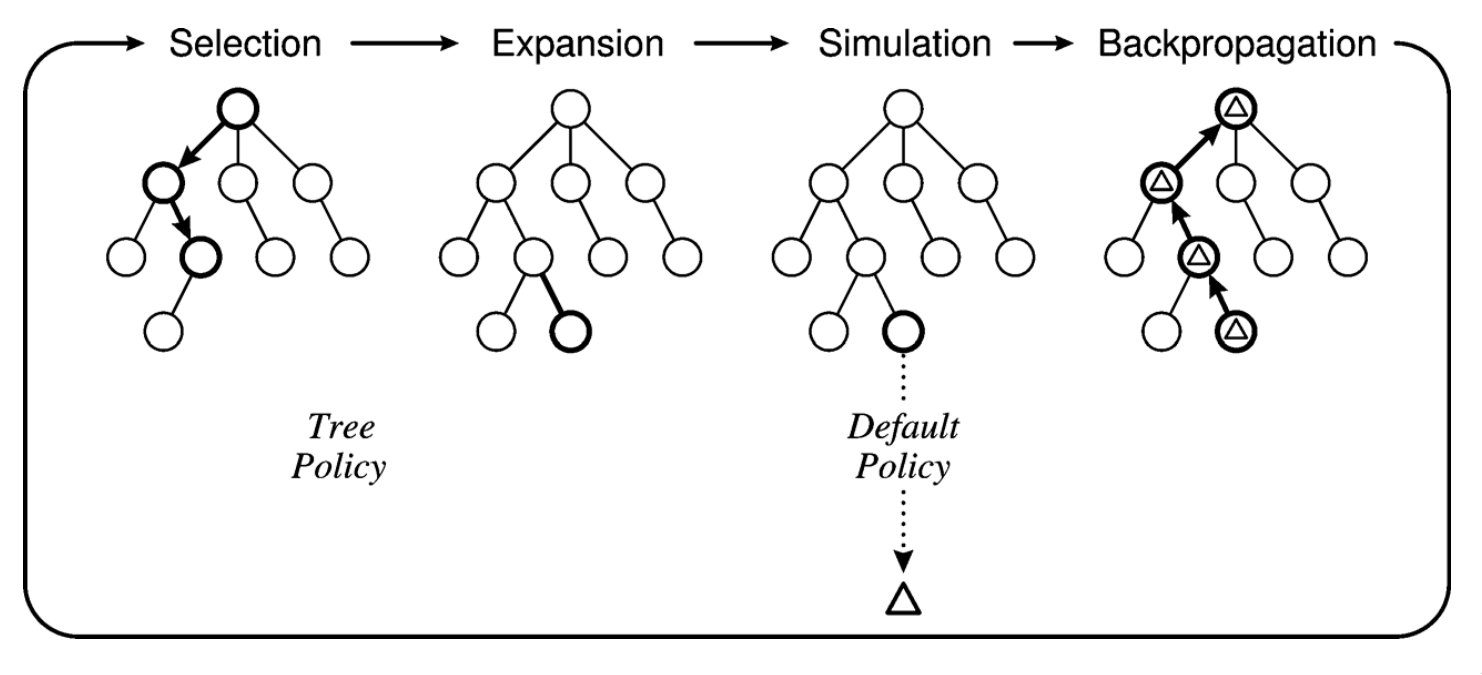
\includegraphics[width=0.8\linewidth]{mcts-general.png}
  \caption{One iteration of the general \ac{mcts} approach
  \cite{browne2012survey}.\todo[inline]{Selection should be called search.
  Simulation should be called Rollout (to be consistent with
  \cite{kochenderfer2015decision}). Draw this in Inkscape.}}
  \label{fig:mcts-general}
\end{figure}

\subsubsection{Double Progressive Widening}

For problems with large or continuous the state and action space, standard
\ac{mcts} as presented in the previous section will produce very shallow trees.
In fact, if the action space is infinite (e.g. continuous or countably
infinite), \ac{mcts} using \ac{uct} will never choose a previously expanded
action at the same state node a second time. This is evident from
\cref{eqn:ucb}. For any unexplored action ($N(s, a) = 0$) the second term is
understood to be unbounded, causing the tree policy to favor untried actions.
Additionally, if the state space is continuous and the transition probability
density is finite, the event of $G$ generating the same state twice has
probability zero. As a result, simulated trajectories will never pass through
the same state node, causing the policy tree to never expand beyond the first
layer.

Progressive widening addresses this issue by artificially limiting the number
for children of a node to $kN^\alpha$, where $N$ is the number of times the
parent has been visited and $k$ and $\alpha$ are problem specific tuning
parameters \cite{couetoux2011continuous}. Originally, this strategy has been
applied to the action space, as described in \cref{alg:aprogwiden}. \acf{dpw}
extends this idea to additionally apply to $\sspace$. In either case, if the
number of children at a node exceeds the progressively incremented limit
(\cref{alg:aprogwiden:lin:check}), instead of generating a new child, one of
the previously generated nodes is selected. By this means, \ac{mcts} expands to
deeper layers earlier and widens the tree as additional iterations are run.
This results in less myopic policies for problems with large state and action
spaces \cite{couetoux2011continuous}.

\begin{algorithm}
  \caption{Progressive widening applied to $\aspace$ \cite{sunberg2018online}.}\label{alg:aprogwiden}
  \begin{algorithmic}[1]
      \Procedure {ActionProgWiden}{$h$}
          \If{$|C(h)| \leq k_a N(h)^{\alpha_a}$}\label{alg:aprogwiden:lin:check}
              \State $a \gets \Call{NextAction}{h}$
              \State $C(h) \gets C(h) \cup \{a\}$
          \EndIf
          \State $\textbf{return } \underset{a \in C(h)}{\argmax}\, Q(ha) + c \sqrt{\frac{\log N(h)}{N(ha)}}$
      \EndProcedure\vspace{10pt}
  \end{algorithmic}
\end{algorithm}

\subsubsection{POMCPOW Algorithm}

The algorithmic procedure for \ac{pomcpow} fundamentally resembles the idea of
\ac{mcts} with a set of modifications for application in the \ac{pomdp} domain.
Instead of reasoning over state-action sequences, the policy tree spans over
action-observation trajectories starting from the initial belief, $b_0$. In
contrast to \ac{pomcp}, \ac{pomcpow} uses \ac{dpw} to focus search on
a progressively expanded set of actions and observations \cite{silver2010pomcp,
sunberg2018online}. This enhancement allows to yield deeper and more richly
sampled policy trees even in the case of large action and observation spaces.
Finally, since \ac{dpw} constraints the set of considered observations, the
algorithm uses a weighted particle collection to represent the outcome
statistics at observation nodes. By this means, the outcome of the generative
model can be fixed to fall inside the allowed set to avoid sample rejection,
while the weighted belief update prevents an erroneous distribution shift.

A detailed pseudo code representation of the algorithmic procedure is provided
in \cref{alg:pomcpow}. With the preceding introduction of \ac{mcts} and the
aforementioned outline of the algorithms key ideas in mind, we proceed by
discussing each subroutine in greater detail.

In addition to the variables defined in the previous sections, we introduce the
following notation to describe the \ac{pomcpow} algorithm: $h$ represents
a history, ($b_0$, $a_1$, $o_1$, $a_2$, \dots, $a_k$, $o_k$), as introduced in
\cref{sec:pomdp}, $ha$ and $hao$ are shorthand for concatenation of $h$ with
$a$ or $(a, o)$, respectively. $d$ denotes the remaining depth to explore, with
$d_\text{max}$ the maximum depth; $C(h)$ is the list of children of node $h$;
$N(h)$ denotes the number of visits of node $h$; $M(hao)$ is a count for the
number of times the observation terminated history $hao$ has been sampled by
the generative model, $G$. $B(h)$ represents a list of states associated with
node $h$, with $W(h)$ the corresponding weights.

\textbf{Plan}\\
The \textsc{Plan} procedure represents the outer loop of the algorithm. Input
to the function is the current belief, $b$, as obtained from a belief updater.
Typically, $b$ is the output of a particle filter. Starting at $b$, the
algorithm performs $n$ iterations of \ac{mcts} to obtain a local approximation
the action value function, $Q$. The procedure is parametrized with
$d_\text{max}$, the maximum search depth of the policy tree. Finally, the planner
selects the action, that maximizes the obtain \qfunction approximation.

\textbf{Simulate}\\
The \textsc{Simulate} procedure resembles a recursive implementation of
a single \ac{mcts} iteration. Inputs to the function are a sampled state, $s$,
an action-observation history as introduced in \cref{sec:pomdp}, $h$, as well
as the remaining search depth, $d$. Unless the maximum depth is reached, the
algorithm proceeds by selecting an action $a$ using action progressive
widening. Given this action, a state-observation-reward tuple is sampled from
the generative model. Subsequently, observation progressive widening
(\crefrange{alg:lin:oprogwide_start}{alg:lin:oprogwide_end}) is applied to
either generate a new observation and increment the corresponding counter, or
sample one of the previously generated observations, $o \in C(ha)$. The
generated state, $s'$, is added to the state list at the observation node,
$B(hao)$. In order to resemble a weighted particle belief, the corresponding
weight is chosen according to the observation model, $\odist(o \mid s, a, s')$,
and is stored in the associated weight vector, $W(hao)$.

If the observation is not a child of this action terminated history node, a new
observation node is created and a rollout in the spirit of \ac{mcts} is
performed. Otherwise, search on the partially constructed policy tree continues
one level deeper by sampling a state, $s'$, from the weighted particle
collection to proceed with the next \textsc{Simulate} recursion.

Finally, backpropagation is performed by passing the simulated \vname{total}
reward up the recursion stack and updating the \qfunction approximation
accordingly.

\begin{algorithm}[H]
    \caption{POMCPOW \cite{sunberg2018online}.}\label{alg:pomcpow}
    \begin{algorithmic}[1]
        \Procedure{Plan}{$b$}
            \For{$i \in 1:n$}
                \State $s \gets \text{sample from }b$
                \State $\Call{Simulate}{s, b, d_\text{max}}$
            \EndFor
            \State $\textbf{return } \underset{a}{\argmax}\, Q(ba)$
        \EndProcedure\vspace{10pt}

        \Procedure {Simulate}{$s$, $h$, $d$}
            \If{$d = 0$}
                \State \textbf{return} $0$
            \EndIf
            \State $a \gets \Call{ActionProgWiden}{h}$
            \State $s',o,r \gets G(s,a)$
            \If{$|C(ha)| \leq k_o N(ha)^{\alpha_o}$}\label{alg:lin:oprogwide_start}
                \State $M(hao) \gets M(hao) + 1$
            \Else
                \State $o \gets \text{select } o \in C(ha) \text{ w.p. } \frac{M(hao)}{\sum_{o} M(hao)}$
            \EndIf\label{alg:lin:oprogwide_end}
            \State $\text{append } s' \text{ to } B(hao)$ \label{lin:insert}

            \State $\text{append } \odist(o \mid s, a, s') \text{ to } W(hao)$ \label{lin:weight}
            \If{$o \notin C(ha)$}
                \State $C(ha) \gets C(ha) \cup \{o\}$
                \State $total \gets r + \gamma \Call{Rollout}{s', hao, d-1}$
            \Else
                \State $s' \gets \text{select } B(hao)[i] \text{ w.p. } \frac{W(hao)[i]}{\sum_{j=1}^m W(hao)[j]}$ \label{lin:sample}
                \State $r \gets \reward(s,a,s')$
                \State $total \gets r + \gamma \Call{Simulate}{s', hao, d-1}$
            \EndIf
            \State $N(h) \gets N(h)+1$
            \State $N(ha) \gets N(ha)+1$
            \State $Q(ha) \gets Q(ha) + \frac{total - Q(ha)}{N(ha)}$
            \State \textbf{return} $total$
        \EndProcedure\vspace{10pt}
    \end{algorithmic}
\end{algorithm}

\missingfigure{graphical model of POMCPOW-Tree with weighted scenarios.}

\section{Tools and Software Framework}

Solving a \ac{pomdp} poses a challenging problem from both, the
implementational\todo{is this the right phrasing?} and computational
perspective. Therefore, suitable software tooling is required that provides
a simple but expressive way of describing problems and solvers while leveraging
the full computational power of the hardware involved.

This section briefly discusses the tooling choices made for the experiments
conducted throughout this work. This discussion is not thought to be a detailed
comparison of \ac{pomdp} frameworks but rather seeks to provide insight into
how the tools used here can help to accelerate the solution process.

To date, there exist a number of frameworks that are capable of solving
sequential decision making problems under uncertainty, some of which also
accommodate partially observable domains. In this work we make use of the novel
framework \pomdpsjl, an open-source interface for solving \acp{mdp} and
\acp{pomdp} \cite{egorov2017pomdps}. Unlike other popular frameworks like APPL
(\cite{appl}), AI-Toolbox (\cite{aitoolbox}), and ZMDP (\cite{zmdp}), \pomdpsjl
is not written in \emph{C++} but in the \emph{Julia} programming language. This
enables the user to flexibly build prototypes while the high-performance nature
of the language allows to scale ideas to run extensive simulations on large
multi-node clusters. Benchmarks in the past have shown that despite being
a high-level language that abstracts a lot of complexity, the execution time of
code written in \emph{Julia} can still compete with \emph{C++} implementations.
In fact, experiments we ran to evaluate the runtime for one of the problems
studied in \cref{chap:hri} suggest that the highly-optimized code produced by
the \emph{Julia} compiler may even outperform a \emph{C++} implementation,
unless the later is carefully tuned by an experienced software engineer. The
results of this problem specific benchmark can be found in \todo{point to
appendix}.

In addition to the advantages generated by the choice of programming language,
\pomdpsjl provides a simple yet expressive interface to describe, solve and
simulate \acp{pomdp}. The toolbox specifies abstract interfaces for three
conceptual elements: \emph{problems}, \emph{solvers} and \emph{experiments}.
This design decouples these subdomains, thus ensuring that code can be written
for each of them separately while not sacrificing interchangeability. Finally,
the associated \emph{JuliaPOMDP} community provides a number of
state-of-the-art \ac{mdp} and \ac{pomdp} solvers as well as a rich library of
tools for implementing and evaluating solvers and solutions.

\chapter{Simultaneous Localization and Planning}\label{chap:localization-and-planning}

\todo[inline]{Rework according to results}

Typically, robot localization and motion planning are treated as mostly
independent tasks. Often, the problem provides the agent with a focused initial
belief or allows the agent to quickly reduce uncertainty by first collecting
a series of measurements that don't require elaborate motion planning. This is
particularly the case if the state space is well observed, i.e. there exists
a sensor that provides the robot with a (noisy) position reading (e.g. GPS).
For these well behaved problems, a simple yet effective approach is to first
collect sensor data while executing a default motion, i.e. rotating about the
yaw axis to collect measurements in all directions. Once state uncertainty is
reduced to a focused, unimodal belief, the problem is treated as fully observed
problem and motion planning is performed on expectation. That is, trajectories
are planned based on the assumption that the expectation of the belief, $E[b]$,
is a sufficient approximation for the true position of the robot. Furthermore,
higher statistical moments \todo{What is the right word for this?} may be used
to trigger additional information gathering. In even simpler problems, plan
execution may implicitly yield sufficient information gathering, rendering
explicit consideration of this aspect obsolete.

However, more challenging problems are obtained when information gathering
happens less naturally. In these cases, a simple approach as outlined above
may not perform well. Instead, persistently good performance requires the agent
to consider the full belief distribution as well as future observations in
order to identify informative action sequences.

\todo[inline]{Rewrite once structure (below) has converged}
An instance of such problem is studied in this chapter. We begin by stating the
problem details in \cref{sec:lp-problem-statement}.
\cref{sec:lp-pomdp-formalization} then formalizes this problem as a \ac{pomdp}.
\cref{sec:lp-solutions} presents solution strategies based on \ac{pomdp}
solvers introduced in \cref{sec:online-pomdp-solvers} as well as two heuristic
baseline approaches. Finally, we evaluate the performance of each solver and
discuss the results \cref{sec:lp-evaluation}.

\section{Problem Statement}\label{sec:lp-problem-statement}

Consider a robot operating in a planar, previously mapped room as depicted in
\cref{fig:roomba-env}. In this figure the red marker denotes the true position
of the robot, while the blue particles represent the robot's belief of it's
current location in the room. The agent is tasked to reach the exit (green)
while avoiding falling down the stairs (red). Additionally, unnecessary
collisions are to be avoided. The scene shows the simulation in it's initial
configuration: The robot starts at a position drawn uniformly at random from
the set of all possible position-orientation tuples. This initial position is
not known by the agent, thus the particles representing the initial belief are
spread uniformly across the entire room. The robot is equipped with a single
sensor that provides information about collisions with walls of the room. The
robot's dynamics are governed by an underactuated first-order model that allows
the robot to translate forward and/or rotate about it's vertical axis. The
agent holds control authority to choose translation and rotation rates.

This problem has originally been published under the name \emph{"Escape
Roomba"} by the \emph{Stanford Intelligent Systems Laboratory} as part of the
class \emph{Decision Making under
Uncertainty}\footnote{\url{https://web.stanford.edu/class/aa228/cgi-bin/wp/}}.
The experiments presented in the following have been conducted using the
\pomdpsjl implementation of the
problem\footnote{\url{https://github.com/sisl/AA228FinalProject}}.

\begin{figure}[htpb]
  \centering
  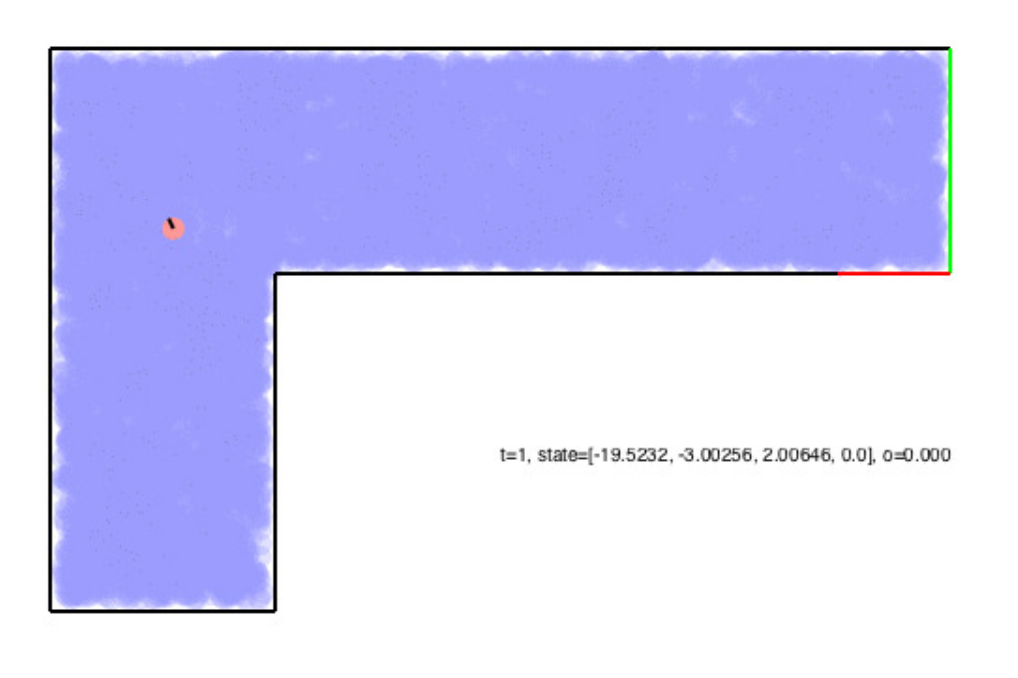
\includegraphics[width=0.7\textwidth]{roomba_demo/roomba-initial.png}
  \caption{A screen shot of the simulation environment for the \emph{"Escape
  Roomba"} problem provided by the \emph{Stanford Intelligent Systems
  Laboratory} as part of the class \emph{Decision Making under Uncertainty}.}
  \label{fig:roomba-env}
\end{figure}

\clearpage
\section{POMDP Formalization}\label{sec:lp-pomdp-formalization}

The problem is formalized as a \ac{pomdp} with the following properties introduced in \cref{sec:pomdp}:

\todo[inline]{Mention somewhere that we discretize the action space because
samples are expensive (problem setup is quite slow)}

\begin{description}
	\item[State Space $\sspace$.] The state of the robot is defined as the
	position, orientation tuple, $s=((x,y), \alpha)$. Respectively, $\sspace$ is
	the set of all positions-orientation tuples inside the room.
	\item[Action Space $\aspace$.] An action is defined as a translation-rotation
		rate tuple, $a=(v, \omega)$. $\aspace$ is the set of all these
		tuples adhering to the physical limitations of the system.
  \item[Transition Model $\tdist$.] The robot transition flows the dynamics of
    a simple differential drive model. The details of this transition are
    defined implicitly by the simulator and are treated as a generative black
    box model.
  \item[Reward Function $\reward: \sspace \times \aspace \times
    \sspace \to \reals$.] The reward model is defined as:
    \begin{equation}
      \reward(s, a, s') = r_\text{time} + \chrond(s') r_\text{collision} + \chrond(s') r_\text{goal} + \chrond(s') r_\text{stairs}.
    \end{equation}
    Here, $\chrond_\text{c}(s)$ denotes the \vname{Kronecke delta} function under the condition, \vname{c}, such that
    \begin{equation}
      \chrond_\text{c}(s) = \begin{cases}
        1, & \text{if condition $c$ holds for $s$}\\
        0, & \text{otherwise.}
      \end{cases}
    \end{equation}
    The reward model is parametrized by the following
    quantities: $r_\text{time}$ is a living penalty encouraging the robot to
    minimize the time until the goal is reached; $r_\text{collision}$ is
    a penalty for collision with walls; $r_\text{goal}$ is the reward obtained
    when reaching the goal, and $r_\text{stairs}$ the penalty for falling down
    the stairs.\\
  \item[Discount Factor $\gamma$.] Rewards are discounted with $\gamma = 0.99$.
  \item[Observation Space $\ospace$.] The sensor provides a binary output,
    stating whether the robot is currently in contact with the wall or not. That
    is, there are only two observations: $o^0$  and $o^1$.
  \item[Observation Model $\odist$.] The collision sensor is deterministic.
    That is, the observation model is a Dirac delta function, evaluating
    non-zero for a state, $s$, if and only if the collision feature evaluated
    on $s$ matches the observation, $o$.
\end{description}

Summarizing, the problem is a \ac{pomdp} with continuous state and action space
and a discrete observation space. The reward model chosen for this problem is
sparse. That is, it only encodes high level preferences but avoids biasing the
solution through additional transition dependent rewards (e.g. rewards for
reducing the distance to the goal).

\section{Solution Strategies}\label{sec:lp-solutions}

We solve the \ac{pomdp} described in \cref{sec:lp-pomdp-formalization} using
\ac{despot} and \ac{pomcpow}, respectively. For each of these solvers we
propose two domain specific adaptations to guide the policy search. In addition
to that, we present two baseline policies that use a heuristic policy to
control the agent. In order to consider efficiency of each algorithm we limit
the computation time per planning step to $T_\text{max} = \SI{1}{s}$. Each
policy uses the same particle filter to estimate the root belief.
\todo[inline]{Maybe point to code attached or to repo.}

\subsection{Baseline Policies}\label{sec:lp-baseline}

In order to obtain a baseline we make a common simplifying assumption: Instead
of planning with the full root belief, $b$, the policy uses only the \emph{most
likely state}, $\sml = \mode(b)$. Using this approximation, the problem is then
treated as fully observable. That is, at every time step the control action is
selected based on the assumption that the true position of the robot matches
the most likely state. The loop is closed by applying only the first action of
the policy at each time step to then update the belief and re-plan from the
next most likely state, $\sml' = \mode(b')$. Based on this assumption we
propose two heuristic policies:

\begin{description}
  \item[\ac{mlra}] For this baseline, the agent uses a simple, handcrafted
  feedback policy that does not involve any active reasoning about future
  states. Instead, it uses a proportional controller to track the center line
  of the room to reach exit. As a result, evaluating \ac{mlra} is
  computationally inexpensive. \ac{mlra} is not an optimal policy for the fully
  observable problem.
  \item[\ac{mlmpc}] This planning agent computes the optimal state trajectory
  for the fully observable problem starting from $\sml$. That is, it uses the
  negative reward model as a cost function to obtain the objective for the
  model predictive controller.
\end{description}

Unlike \ac{mlra}, \ac{mlmpc} is an optimal policy for the fully observed
problem. However, it should be noted that this result does not necessarily
translate to the partially observed domain. Appendix TODO\todo{cref to
appendix} compares the performance of both baseline policies for the fully
observable case.

\subsection{POMDP Solvers}\label{sec:lp-planners}

We use \ac{despot} and \ac{pomcpow} to solve the \ac{pomdp}. For each solver we
propose two strategies in which domain knowledge can be utilized to guide the
policy search for the localization and planning problem.

\subsubsection{DESPOT}\label{sec:lp-planners-despot}

As presented in \cref{sec:theory-despot}, \ac{despot} uses upper and lower
bounds, $U_0$ and $L_0$, on the value function to guide the policy search and
prune the determinized policy tree. In theory, the tighter these bounds are on
the true value function, the more efficiently the algorithm will focus on
exploring the relevant trajectories. On the other hand, if these estimates
violate the true bounds on the optimal cost to go, \ac{despot} with perform
sub-optimally. However, as proven in \cite{somani2013despot}, the algorithm is
robust against approximation errors. That is, similar to informed graph search
algorithms like \emph{A*}, the performance of the algorithm will degrade
gracefully with violations of $U_0$. In fact, similar to bounded relaxations of
\emph{A*}, non-admissible heuristics may help to find good solutions earlier.
Therefore, even if $U_0$ is not a true upper bound on the optimal value, it may
help to improve performance when limited planning time does not allow to
thoroughly explore the search space. Furthermore, it should be noted that
finding tight bounds at the expense of high compute also defeats the purpose.
In the limit, finding the tightest upper and lower bound on the optimal value
requires solving the entire \ac{pomdp}. Therefore, choosing suitable upper and
lower bounds is an important design choice when adapting \ac{despot} for
a specific problem.

There exist a variety of strategies to compute these upper and lower bounds.
\todo{maybe list some common ones}
In the following we present two of the strategies we found most effective for
the problem studied here.
\todo[inline]{point to the code on the cd (or appendix)}

\begin{description}
  \item[Analytic Bounds] In this strategy we compute the bounds using an
    analytic, closed form\todo{what is a better phrasing for this?}
    approximation for $U_0$ and $L_0$. Due to the structure of the reward
    model, we can directly compute the cumulative reward for an arbitrary
    $n$-step, collision-free trajectory. Let $\hat{\Sigma}: \naturals \to
    \reals$ be this mapping. We compute the upper bound, $U_0$, on the optimal
    value by considering a strict relaxation of the problem: First, we assume
    that the robot is located at the closest position to the goal out of all
    particles in the current belief; Second, we assume that the robot can
    immediately move on a straight line to the target. With this relaxation we
    compute the minimum remaining number of steps, $n_{\text{min}}$, from the
    minimum Euclidean distance over all particles to the goal and the maximum
    translational speed. For the lower bound, $L_0$, we proceed in
    a similar fashion. In this case, however, we consider the worst case
    particle by using the $\ell_1$ norm as a distance metric combined with an
    under-approximation on the velocity to obtain $n_{\text{max}}$. In either
    case, we use $\hat{\Sigma}$ to map the step estimate to a corresponding
    return. Using these approximations, $U_0$ is a true upper bound on the
    optimal value. While for $L_0$ there is no strict guarantee to be a true
    lower bound, we found that most cases it is well behaved.
  \item[Rollout Lower Bound] This strategy uses the same upper bound as the
    first approach. However, for $L_0$ we use a default policy rollout to
    obtain a true lower bound. In order to generate a structured motion, we use
    a \emph{fixed-action} policy that always selects the forward action,
    instead of the common random policy rollout. By this means, the rollout
    policy provides a tight lower bound once evaluated from a state that
    already faces the exit of the room.
\end{description}

\subsubsection{POMCPOW}\label{sec:lp-planners-pomcpow}

\ac{pomcpow} uses a value estimate to approximate the remaining reward to be
collected from a leave node of the policy tree. Due to the design of the
algorithm, this value estimate is only ever invoked on observation nodes when
visited for the first time (cf. \cref{alg:pomcpow}). As a result, the
corresponding belief consists of only a single state and the problem is de
facto fully observable. Hence, in order to adapt this algorithm for a specific
problem one can design the value estimate based on the corresponding \ac{mdp}.
Hereafter, we present two strategies strategies to compute this value estimate
for the localization and planning problem.

\begin{description}
  \item[Analytic Value Estimate] We compute an analytic value estimate for
    state, $s$, with a strategy similar to the one used to obtain analytic
    bounds for \ac{despot}. We relax the planning problem by assuming that the
    robot can move immediately from $s$ to the goal on a rectilinear
    trajectory. Using this relaxation we can compute the estimate on the
    remaining number of steps to the goal, $\hat{n}$. We then obtain the value
    estimate for an $\hat{n}$-step, collision-free trajectory by propagating
    $\hat{n}$ through $\hat{\Sigma}$, introduced above.
  \item[Rollout Estimate] A commonly used strategy in \ac{mcts} is a random
    policy rollout \cite{browne2012survey}. For this problem, however, random
    play-outs do not provide a good value estimate since random trajectories
    will often fail to reach a terminal state within reasonable time. Instead,
    we use the \emph{fixed-action} policy proposed for the \ac{despot} lower
    bound approximation in the preceding paragraph.
\end{description}

\section{Evaluation}\label{sec:lp-evaluation}

We evaluate the performance of each strategy by running $N_\text{sim} = 1000$
simulations for every setup. In an effort to reduce sampling variance, we
initially fix $N_\text{sim}$ random seeds. These seeds are shared across the
different setups for a fixed run. By this means, the $i$th run of each setup
will see the same random outcome (i.e. same initial conditions and noise
trajectories, etc.). In order to handle cases in which the agents fails to
reach a terminal state in a reasonable amount of time, each simulation is run
for a maximum of number of time steps, $T_\text{max,sim} = 300$. The choice of
this upper bound on simulation time is justified by evaluation of the optimal
policy for the fully observable problem. In the corresponding \ac{mdp} with the
same set of initial conditions, \ac{mlmpc} reached the goal within a maximum
number of $56$ over all scenarios. Therefore, it is reasonable to assume that
a well behaved policy for this \ac{pomdp} should be able to reach a succeeding
terminal state within a time horizon more than five times longer than the worst
case fully observable run.

We begin by comparing the performance of each strategy by examining the
cumulative discounted reward. Since maximizing the sum of discounted rewards is
the objective function for this optimization function, this is the most natural
benchmark. In order to account for the reward discarded in cases where
$T_\text{max, sim}$ is exceeded, we penalize the value of these runs by
extrapolating the living penalty over infinite horizon. Since the sum over the
infinite sequence of discounted rewards is geometric series, we obtain the
closed form solution,
\begin{equation}
  r_{T_\text{sim,max}} = \sum_{t=1}^\infty r_\text{time} \gamma^{t-1} =  r_\text{time} \frac{\gamma}{1-\gamma}.
\end{equation}
Since this reward is collected at the end of the simulation horizon it must
discounted accordingly, entering the objective function as
\begin{equation}
  \Delta V_{T_\text{max,sim}} = r_{T_\text{sim,max}} \gamma^{(T_\text{max,sim} - 1)}
\end{equation}
Following this argument, with the parameters chosen for this problem an agent
that does not reach a terminal state within the simulation horizon is penalized
with $\Delta V_{T_\text{max,sim}} = -0.49$.

\Cref{fig:lp-value-sem-inf-discounted} shows the mean and \ac{sem} of the cumulative
discounted reward for $1000$ experiments over each policy. The \ac{sem}
approximates the standard error between the empirical mean obtained from the
sampled experiments and the true mean of the distribution, obtained
hypothetically for $N_\text{sim} \to \infty$. The results shows that under this
metric all \ac{pomdp} planners perform significantly better than the baseline
policies. Within the baselines the planning agent (\ac{mlmpc}) performs better
than the proposed reflex agent (\ac{mlra}). Out of all \ac{pomdp} planners
\ac{pomcpow} with analytic value estimate achieves the best results. Furthermore,
notice that \ac{despot} shows approximately the same performance for both bound
approximations while for \ac{pomcpow} the analytic value estimate shows a yields
improvement.

\begin{figure}[H]
  \centering
  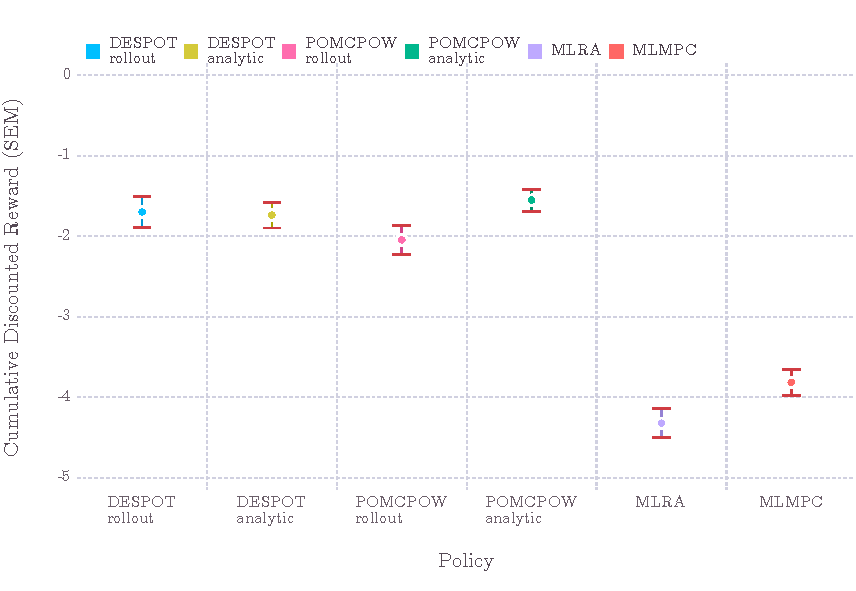
\includegraphics[scale=1.0]{roomba_plots/lp_value_sem_eval_plot-inf_discounted_reward.pdf}
  \caption{Mean and \acf{sem} for each policy introduced in \cref{sec:lp-solutions}.}
  \label{fig:lp-value-sem-inf-discounted}
\end{figure}

Further insight is gained by looking at the distribution of returns for each
policy. \Cref{fig:lp-value-violin-inf-discounted} shows an approximation of the
probability density function for the value distribution based on the $1000$
samples for each policy. From this visualization another important difference
becomes apparent. While the mean performance of all \ac{pomdp} planners is
approximately the same, those versions of \ac{despot} and \ac{pomcpow} using an
analytic strategy for bound and value approximation manage to reduce the lower
tail end of the distribution. As a result, these planners show less variance in
performance than solvers using the corresponding rollout estimates.

\begin{figure}[H]
  \centering
  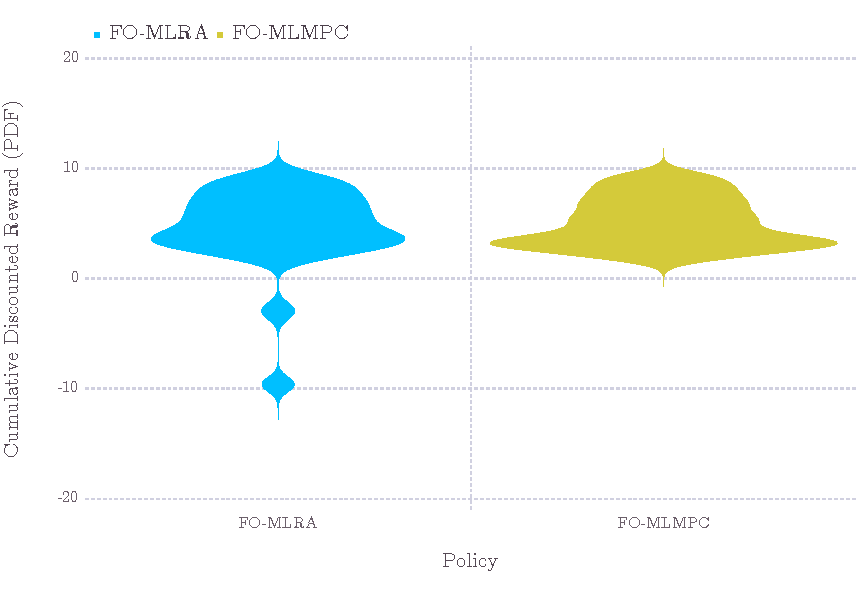
\includegraphics[scale=1]{roomba_plots/lp_value_violin_eval_plot-inf_discounted_reward.pdf}
  \caption{Approximation of the \acf{pdf} for the value distribution gained by each policy.}
  \label{fig:lp-value-violin-inf-discounted}
\end{figure}

These quantitative results also manifest in the qualitative performance of each
policy. When looking at trajectories generated by each solver, we notice that
the \ac{pomdp} planners typically generate trajectories that efficiently
eliminate a lot of uncertainty. The baseline strategies on the other hand only
passively reduce uncertainty by colliding with wall if the mode of the belief
is located in cluster far away from the true position of the robot. For many
cases this kind of passive information gathering is strong enough to help the
robot eventually reach it's goal. However, we notice that for certain
typologies of the belief the baseline policies fail to reduce uncertainty, e.g.
if the belief is highly symmetric. In these cases, often slight modifications
of the trajectory would have been sufficient to break symmetry and completely
eliminate a cluster. While \ac{despot} and \ac{pomcpow} are able to actively
identify information gathering strategies for these cases, the baseline
policies often oscillate until repeated re-sampling in the particle filter
breaks the symmetry to an extent that allows to stabilize decisions.

Furthermore, one can observe that all \ac{pomdp} planners are significantly
better at avoiding failures (falling down the stairs). If the planner is
presented with a belief that features a cluster near the stairs, the agent
typically chooses a sequence of actions that is safe for this hypothesis and
reduces uncertainty in this regime to avoid entering the failing terminal
state. Since the baselines consider only the most likely state, these policies
fail when the topology of the reward is such that this state is facing
the goal while the true position -- guided by particles with a smaller
likelihood weight -- is facing the stairs.

Finally, we observe that the \ac{pomdp} planners using a rollout strategy to
guide the search behave more myopic. While shortsighted planning still allows
the agent to be robust against falling down the stairs, these policies tend to
get stuck when a long sequence of actions is required to eliminate uncertainty.
A possible reason for this is the fact that rollouts are more computationally
expensive than analytic bound and value estimates. Additionally, in these
regimes the fixed-action rollout typically does not provide a tight lower bound
or accurate value estimate for \ac{despot} and \ac{pomcpow}, respectively. In
the case of \ac{despot}, even though the sparse approach most likely allows
some branches of the tree to be constructed to full depth, the loose lower
bound causes policy search to be poorly guided while the limit planning time
does prevents sufficient exploration of more promising branches. In the case of
\ac{pomcpow} the computationally expensive rollout performed for every iteration
of the algorithms hinders the policy tree to reach sufficient depth within
the computation budget. Since rewards are sparse, on a short horizon all
futures appear to provide similar reward. Hence, \ac{despot} and \ac{pomcpow}
fail to identify a promising strategy within their mostly shallow policies trees.

\todo[inline]{Maybe have some figures with sequences of frames and beliefs to show
what the agent does.}

Summarizing the results of this qualitative analysis,
\emph{\ac{despot}-analytic} and \emph{\ac{pomcpow}-analytic} generate highly
efficient and robust behaviors. All other policies show weaker with different
kinds of failure modes: The rollout versions of the \ac{pomdp} planners more
often fail to reach the exit due to myopia but still show good performance when
it comes to avoiding failure states; \ac{mlmpc} rarely fails to reach the goal
state but often takes very long or becomes unlucky when greedily tyring to
reach the exit; \ac{mlra} shows an overall worse performance than all other
policies.

These results are additionally confirmed when evaluating metrics other than the
objective of the optimization problem. \Cref{fig:lp_outcome} shows
a histogram of the outcome statistics for each policy. We distinguish between
three classes of outcomes: \emph{success (+)}, the robot reached the exit;
\emph{failed to exit (0)}, the agent did not make it to the exit within the
simulation horizon; and \emph{failure (-)}, the robot fell down the stairs.

\begin{figure}[htpb]
  \centering
  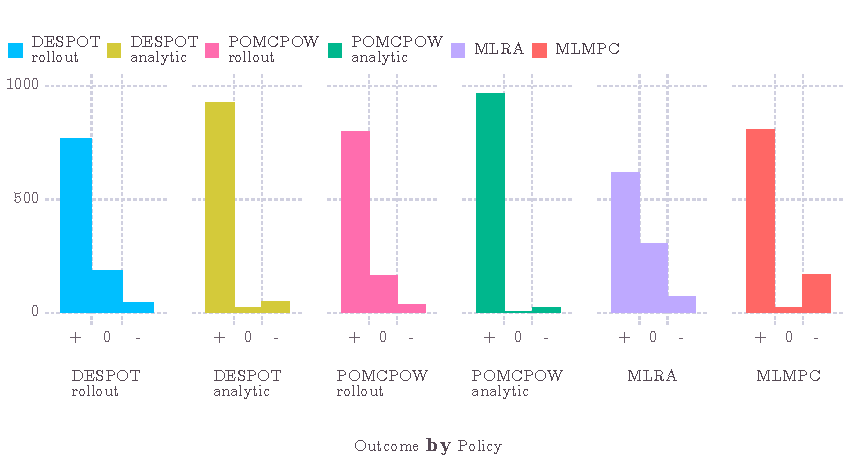
\includegraphics[scale=1.0]{roomba_plots/lp_outcome_eval_plot.pdf}
	\caption{Histogram of the outcome frequencies grouped by policy. Outcome
			     classes: \emph{success (+)}, the robot reached the exit; \emph{failed to
				   exit (0)}, the agent did not make it to the exit within the simulation horizon;
		 	 	   and \emph{failure (-)}, the robot fell down the stairs.}
	\label{fig:lp_outcome}
\end{figure}

Additional evidence for the findings discussed above is provided by the
statistics of the \emph{cumulative undiscoutned reward}. While this metric does
not match the objective for the inifinite horizon formulation, it may match the
perceived \emph{qualitative performance} more closely since we can only observe
the agent for a finite time horizon. \Cref{fig:lp_eval_undiscounted} show the
\ac{sem} and \ac{pdf} approximation for the undiscoutned reward sequence. Using this
metric, it becomes clear that the analytic versions of the \ac{pomdp} planners
outperform all other strategies. Here, we can additionally identify a subtile
performance gap between \emph{\ac{despot}-analytic} and
\emph{\ac{pomcpow}-analytic}. In fact, the \ac{pdf} approxiamation of the
cumulative undiscoutned reward show that \emph{\ac{pomcpow}-analytic} manages
to elimite large parts of the low value tail.


\begin{figure}[htpb]
  \centering
  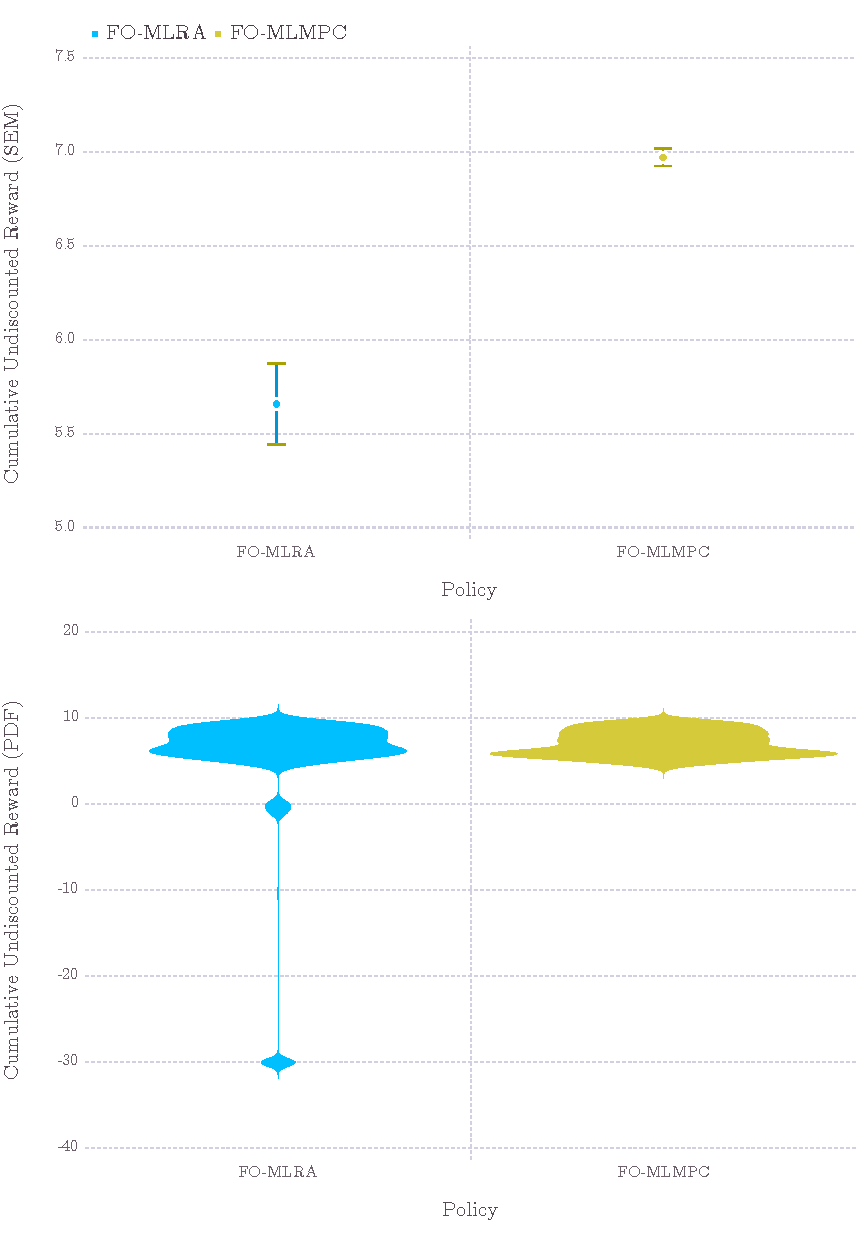
\includegraphics[scale=1]{roomba_plots/lp_value_eval_plot-undiscounted_reward.pdf}
  \caption{Name}
  \label{fig:lp_eval_undiscounted}
\end{figure}

%  \begin{figure}[H]
%    \centering
%    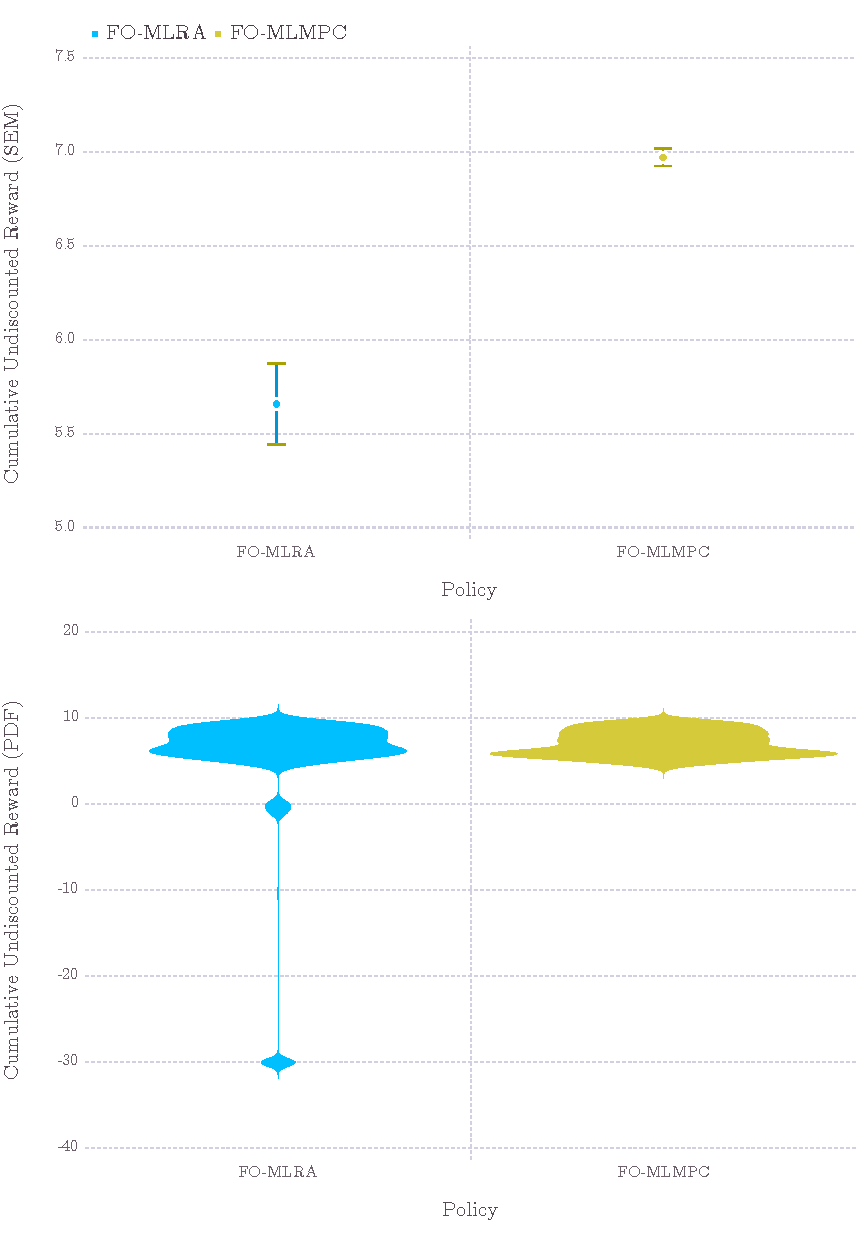
\includegraphics[scale=1]{roomba_plots/lp_value_eval_plot-undiscounted_reward.pdf}
%    \caption{Name}
%    \label{fig:name}
%  \end{figure}

\chapter{Motion Planning with Latent Human Intentions}\label{chap:hri}

Robots that are designed to assist humans almost inevitably have to operate in
a shared environment. \ac{hri} requires autonomous agents to navigate
safely in domains that typically do not feature safety barriers to physically
separate them from humans. Therefore, robots must ensure human safety through
careful planning and robust behaviors. At the same time, trajectories of humans
are hard to predict as they follow complex behaviors whose dynamics are only
partially understood. For this reason, research in the past has moved from
simple rule-based and deterministic models
\cite{helbing1995social,burstedde2001simulation} towards data driven
probabilistic predictions that approximate the future as a distribution over
trajectories \cite{kretzschmar2014learning,alahi2016social,gupta2018social}.

% \todo[inline]{Explain the notion of latent, internal state}

Incorporating stochasticity in the prediction pipeline allows the planner to
model uncertainty over both, high-level intentions (e.g. \emph{where} does the
human want to go), and low-level motion behavior (e.g. \emph{how} does the
human want to go there). Planning strategies that take this uncertainty into
account promise to provide robustified and potentially more efficient policies
for navigation around humans. While the properties gained from this kind of
planning are desirable for many \ac{hri} problems, reasoning over distributions
of possible futures may pose a challenging \ac{pomdp}. Therefore, a lot of
research has focused on recovering some of these properties by proposing domain
specific simplifications for these applications \cite{fern2007decision,
sadigh2016information, javdani2018shared, fisac2018probabilistically}.

On the other hand, recent research in this field suggests that through
increased performance of modern solvers, \ac{pomdp} approaches for motion
planning problems with \ac{hri} are becoming increasingly practical and that
this kind of reasoning can help to generate robustified and more efficient
behaviors for this domain. \cite{bai2015intention} use the \ac{despot} to
control the speed of an autonomous golf cart for navigation in a crowd. They
show that by reasoning over future observations the system is able to maneuver
more safely while reaching the goal faster and increasing passenger comfort
through smoother trajectories than the proposed greedy baseline.
\cite{sunberg2017value} examine the value of inferring the internal state of
traffic participants for autonomous freeway driving. The results presented in
their work show that the problem allows for a significant increase in
performance when the agent is omniscient to the individual internal state of
other vehicles compared to planning with a static \emph{normal} behavior for
all traffic participants. They demonstrate that inference of the latent
behavior parameters in combination with \ac{pomdp} planning allows to greatly
reduce the gap to the omniscient upper bound.

While a lot of work in motion planning under uncertainty has focus on either
\emph{problem specific simplifications} on the one hand or \emph{full
\ac{pomdp} solutions} on the other, few results exist on the direct comparison
of the two. In this chapter we consider a case of motion planning in the
presence of humans for which a sophisticated domain specific strategy has been
proposed in \cite{fisac2018probabilistically}. This strategy simplifies the
planning problem by neglecting future observations. Instead, human prediction
are performed on expectation from the current belief, providing series of
probability maps for future human motion. The authors propose a method that
allows planning with these probabilistic predictions by means of conventional
motion planning algorithms. We implement this strategy in the \pomdpsjl
framework to compare its performance with behaviors generated by
\ac{pomcpow}.

We begin by stating the details of the motion planning problem in
\cref{sec:hri-problem-statement}. \cref{sec:hri-pomdp-formalization} then
formalizes this problem as a \ac{pomdp}. \cref{sec:hri-solutions} briefly
presents the domain specific approximate planner proposed in
\cite{fisac2018probabilistically}, as well as the \ac{pomcpow} solver adapted
for this problem. Finally, we evaluate the performance of both policies and
discuss the results in \cref{sec:hri-evaluation}.

\section{Problem Statement}\label{sec:hri-problem-statement}

In this chapter we study a motion planning problem for a robot in a shared
environment with a human actor. The assumptions made for this planning problem
aim to closely match the setup described in \cite{fisac2018probabilistically}.

\paragraph{High Level Problem}

Consider a human and a robot navigating in a common environment. As a running
example, this problem may be envisioned as an indoor navigation problem. In
this problem, the robot aims to efficiently reach a preset goal location
inside the room while trying to avoid collisions with the human. At the same
time, the human does not pay attention to the robot. That is, the decisions of
the human actor do not depend on the location of the robot. Furthermore, the
human has time-varying intentions that are not known by the robot. At every
time step the human aims to reach a certain goal inside the room. Once arrived
at this goal, the human may either stay at this goal or proceed to another goal
location. Furthermore, the human has a small likelihood of changing the
intended walk target mid way. The robot has a model for some of the locations
humans might want to go to. However, the planner neither knows the exact path
the human will take, nor is its model of human goals complete. That is, the
person might aim to reach an unmodeled goal location. At every time step the
robot receives a perfect observation of the current position of both itself and
the human. The robot ultimately needs to plan and execute a trajectory to
a goal state according to some notion of efficiency, while avoiding collisions
with the human.

\paragraph{Human Behavior Model}

This problem poses a challenging planning problem as it requires the agent to
carefully reason about the intentions of the human in order to avoid collisions
while trying to reach its own goal. Furthermore, in order to be robust against
cases in which the person tries to approach an unmodeled goal, the agent needs
to make safe fall-back predictions when the human behaves unexpectedly. At the
same time, planning with the worst case assumption by trying to avoid the
humans forward reachable set is too conservative.

In this problem setting, the robot is assumed to have access to suitable human
reward function. In practice such reward model can be learned offline from
prior human demonstrations, e.g. using inverse reinforcement
learning. By means of a noisy-rationality model used in cognitive
science \cite{baker2007goal}, the planner can make probabilistic predictions
of human actions given the state,

\begin{equation}\label{eq:boltzmann}
  P\left(a^t_\text{H} | s^t_\text{H}; \beta, \theta \right) \propto e^{\beta Q_\text{H}\left(s^t_\text{H}, a^t_\text{H}; \theta\right)}.
\end{equation}

Here, $a^t_\text{H}$ is the human action taken at time $t$; $s^t_\text{H}$ is
the state of the human at this time; $Q_\text{H}(s_\text{H}, a_\text{H}; \theta)$ is the
state-action value function of the human, with $\theta$ being the parameters of the
$Q$-value encoding latent human intentions (e.g. the goal location); $\beta$ is
the so called \emph{rationality coefficient}.\\
This model encodes the assumption that humans are more likely to select actions that
provide a higher $Q$-value. The rationality constant, $\beta$, determines the
degree to which the robot expects the human to align with the provided reward
model. For $\beta = 0$ the model in \cref{eq:boltzmann} degenerates to
a uniform distribution over all actions. For $\beta \to \infty$ the human acts
perfectly rational with respect to the utility model,
$Q_\text{H}$.

Here, we treat both $\theta$ and $\beta$ as latent parameters. That is, the
agent needs to reason over the parameters of the human reward model (e.g. its
current goal) as well as the accuracy of this model.

\section{POMDP Formalization}\label{sec:hri-pomdp-formalization}

The problem is formalized as a \ac{pomdp} from the robot perspective. It is
characterized by the following properties introduced in \cref{sec:pomdp}:

\begin{description}
  \item[State Space $\sspace$.] The state of the environment is defined as the
  joint state of the human and the robot. For clarity, we introduce the
  subscripts $H$ and $R$ to denote the affiliation of a part of the state to
  the human or the robot, respectively. Furthermore, we differentiate between
  \emph{external states} (i.e. state variables that encode physical properties of the
  environment) and \emph{internal states} (i.e. state variables that determine the
  behavior dynamics of an agent), denoted with subscript $E$ and $I$,
  respectively. Using this notation, a state $s$ is composed as:
  \begin{equation}
    s = [s_\text{E,R}, s_\text{E,H}, s_\text{I,H}]^T
  \end{equation}
  It is important to note that, in order to make $s$ Markovian, we need to
  incorporate the internal state of the human. That is, in contrast to a game theoretic
  approach, humans are not explicitly modeled as players taking actions but
  rather in terms of dynamics of the environment. In the model of the robot, the
  human internal state consists of the reward model parameters, $\theta$, and
  the model confidence, $\beta$. The external state of each actor is defined
  by its current position.

  Using this definition of the state, $\sspace$ is the set of all possible
  combinations of positions the human and the robot and the human internal state.
  \item[Action Space $\aspace$.] An action in this problem refers
  \emph{exclusively} to the robot action. At every time step the robot can select
  one of the following six actions:
  \emph{"north", "east", "south", "west", "to goal", and "stay put"}. The
  latter keeps the robot at its current position. All other actions will move
  the agent with constant velocity in the corresponding direction. Here,
  \emph{to goal} is a state dependent action, that is directed straight at the
  robot's goal location. The set of these six actions constitutes the action
  space, $\aspace$.
  \item[Transition Model $\tdist$.] The dynamics of the robot and the human are
    decoupled. Therefore, we can compose the joint state transition from the
    dynamics of each actor. The transition of the robot, $s_\text{R}$ to
    $s_\text{R}'$, depends on the action as described above. The transition of
    the human obeys \cref{eq:boltzmann}. In our model, the human has
    a discretized action space that allows it to stay put or move in one out of
    eight preset directions (i.e. \emph{north}, \emph{north-east},
    \emph{east}...). Hence, at every time step the human action is generated by
    sampling from the generalized Bernoulli distribution obtained from \cref{eq:boltzmann}
    and the human is moved in the corresponding direction. Additionally, the
    transitions of both actors are corrupted by Gaussian process noise. A terminal
    state is reached if either the robot collides with the human or it reaches the goal.
  \item[Reward Function $\reward: \sspace \times \aspace \times
    \sspace \to \reals$.] The reward model of the robot is defined as:
    \begin{equation}
      \reward(s, a, s') = r_\text{time} + \chrond_\text{collision}(s') r_\text{collision} + \chrond_\text{close}(s') r_\text{close}.
    \end{equation}
    The reward model is parametrized by the following quantities:
    $r_\text{time}$ is a living penalty encouraging the robot to minimize the
    time until the goal is reached; $r_\text{collision}$ is a penalty for
    collision with the human or the walls of the room; $r_\text{close}$ is the
    penalty obtained when entering the one-step forward reachable set of the human.\\
  \item[Discount Factor $\gamma$.] Rewards are discounted with $\gamma = 0.99$.
  \item[Observation Space $\ospace$.] At every time step the robot receives an
    exact measurement of the human and itself. That is, the robot gets to observe
    the external state, $s_\text{E}$ of both actors. As a result, $\ospace$ is
    strict subset of the state space.
  \item[Observation Model $\odist$.] Since the position sensor is exact, the observation
    model is a Dirac delta function, evaluating non-zero for a state, $s$, if and
    only if the external state component matches the observation, $o$.
\end{description}

It must be noted that, in order to match the problem statement provided in
\cref{sec:hri-problem-statement}, we consider two slightly different versions
of this \ac{pomdp}. One version is used to represent the dynamics of the simulated
environment, the other is used as a planning model for the robot. This clear
distinction is necessary to encode the modelling assumption that the robot does not
know about all human goals. That is, the robot does not have access to the true
behavior model of the human.

By inspection of the problem formalized above it becomes apparent that the
assumptions made in \cite{fisac2018probabilistically} poses a \ac{momdp} --
a special case of the more general \ac{pomdp}. That is, we can factor the state
into a fully observed part ($s_\text{E}$, the external state) and a partially
observed part ($s_\text{I}$).

% \todo[inline]{Point to the corresponding implementations of these things. This
% is the best way of communicating further details.}

\section{Solution Strategies}\label{sec:hri-solutions}

We solve the \ac{pomdp} described in \cref{sec:hri-pomdp-formalization} using
two different strategies. First, \cref{sec:hri-baseline} presents
\ac{psrp}, a method proposed in \cite{fisac2018probabilistically} that exploits
the special structure of the problem to reduce the computational effort of
solving the full \ac{pomdp}. Thereafter, \cref{sec:hri-planners} presents an
adaptation of \ac{pomcpow} for this problem.

% \todo[inline]{Maybe point to the
% fact that one could also use \ac{despot}, but that we found \ac{pomcpow} to
% work better (data of Andreea) and that the point of this section is rather to
% compare POMDP vs non-pomdp approaches rather than solver internal benchmark.}

\subsection{Probabilistically Safe Robot Planning}\label{sec:hri-baseline}

\acf{psrp} is a method for motion planning with probabilistic predictions.
While an exhaustive discussion of the details of this method is beyond the
scope of this work, we aim to provide insight into the general idea of this
method as a basis for further discussion. For additional information the reader
may refer to the original paper \cite{fisac2018probabilistically}.

\ac{psrp} is designed for a special class of \acp{pomdp} with the following
properties: The problem must be a \ac{momdp} in which the notion of
\emph{immediate safety} can be evaluated solely on fully observed states.
Furthermore, all such state components affecting immediate safety must be
either \emph{actuated} (i.e. directly controlled by the agent) or \emph{fully
decoupled} from the robot dynamics to allow for predictions independent of the
agent's decisions. Both requirements are satisfied for the problem studied in
this chapter: Immediate safety depends only on the position of the human and
the robot, both contained in the \emph{external} (fully observed) part of the
state; Predictions of the human state can be made independently of the robots
trajectory as she ignores the robot position in her decision making process.

The methods exploits these properties to significantly reduce the complexity of
policy search by essentially converting it to an equivalent non-probabilistic
formulation. The converted problem can then be solved using conventional
motion-planning techniques. On an abstract level the algorithmic procedure of
\ac{psrp} performs the following computations to select the next action:

\begin{description}
  \item[Inference / Belief Update] At every time step, the robot receives an
    exact observation of the external state of the environment. These
    observations are used to maintain a belief over the latent parameters of
    the human model presented in \cref{eq:boltzmann}. These are the goal
    location of the human, $\theta$, and the model confidence, $\beta$. The
    exact update of the joint belief takes the form \begin{equation} b'(\theta,
    \beta) \propto P(s_\text{E,H} | s_\text{H}; \theta, \beta) b(\theta,
    \beta). \end{equation} Since the exact Bayesian update is computationally
    demanding, we perform Monte-Carlo integration to run the inference. Note
    that this is a subtle difference to the original implementation, where the
    authors decide the discretize the parameter and state space to obtain
    a tractable update rule.
  \item[Prediction] Using the belief provided by the inference, the agent
    computes a probabilistic prediction of the human position for $K$ future
    time steps. This is done by recursively propagating the particles belief
    through a generative model matching the statistics of \cref{eq:boltzmann}.
    Since the human is modeled to act noisily rational and additionally the
    particle belief represents a distribution over possible human behaviors,
		the prediction introduces uncertainty to the future trajectory of the
		human. That is, while at the current time step the exact position of the
 		human is known from the most recent observation, at future times the
	  robot only has a probabilistic estimate of the person's location.
    An example of such open-loop predictions of the human location is depicted
    in \cref{fig:psrp-prediction-example}. These predictions are used to
    synthesize a probabilistic obstacle map for the next $K$ time steps.
  \item[Planning] The agent uses the $K$ probabilistic obstacle maps obtained
    from the preceding step to compute the optimal sequence of actions for the
    next $K$ time steps. Since the action-space is finite, we use $A^\ast$ to
    solve this policy search problem. We use the negative reward model as
    a cost function to obtain the cost function for the graph search problem.
    Additionally, in line with the idea of \cite{fisac2018probabilistically} we
    prune search nodes for which the collision likelihood exceeds a preset
    threshold, $\varepsilon$.
\end{description}

The result of this computation is applied in the fashion of a $K$-step receding
horizon \ac{mpc}. That is, at every time step the robot only executes the first
action of the optimal action sequence computed above. At the next time step,
all steps are repeated closing the loop over the received observation.

We implement this solver using the \pomdpsjl interface. By this means we can
share the procedures for inference and sampling, thus allowing for a direct
comparison of the solver performance. Our implementation of this algorithm is
carefully optimized for computational efficiency. In particular, we use k-d
trees to perform nearest-neighbor search when checking for collisions of
particles in the belief prediction. Furthermore, we implement an optimized
lightweight graph search library to efficiently solve the policy search
problem. The latter has been published as an open-source Julia
package\footnote{\url{https://github.com/lassepe/GraphSearchZero.jl}} to allow
for usage in other projects.

\begin{figure}[htpb]
  \centering
  \missingfigure{Example of probabilistic predictions}.
  \caption{Example predictions of the human future location in \acf{psrp}.\todo[inline]{Refine caption once figure is finished.}}
  \label{fig:psrp-prediction-example}
\end{figure}

\subsection{POMCPOW}\label{sec:hri-planners}

The \ac{pomdp} formalization presented in \cref{sec:hri-pomdp-formalization}
allows to directly apply \ac{pomcpow} to the problem. To ensure a fair
comparison, the planner uses the same particle filter as proposed for \ac{psrp}
in \cref{sec:hri-baseline} for inference of the latent parameters of the human model.

Considering the insight obtained from the solver comparison discussed in
\cref{chap:localization-and-planning}, we choose to embed domain knowledge
through an analytic value estimate. Using the same kind of reasoning as
discussed in \cref{sec:lp-planners-pomcpow} we approximate the value at the
leaf of the policy tree using a relaxed version of the problem in which the
robot can move on a straight, collision-free line to its goal location. By
means of this relaxation, the value estimate is given as the discounted sum of
living penalties over the remaining steps to the goal.

\section{Evaluation and Discussion}\label{sec:hri-evaluation}

We evaluate the performance of each strategy by running $5000$ simulations for
each policy. Again, each policy is simulated on the same set of random seeds to
reduce sampling variance. Additionally, in an effort to obtain a comparison
that focuses on safety critical situations, we only consider scenarios in which
a naive \emph{straight-to-goal} policy is not successful. We create these
scenarios by sampling initial conditions from uniform prior and reject all
samples for which the simulated naive policy allows the robot to reach its goal.

In contrast to the experiments presented in
\cref{chap:localization-and-planning}, we don't explicitly set an upper bound
on the decision time per step for \ac{pomcpow} but fix the number of
\ac{mcts} iterations instead. We choose the number of iterations by evaluating the
performance of \ac{pomcpow} over a sequence of parameters and select the number
of iterations beyond which saturation is observed. Furthermore, for the
experiments discussed we are able to simulate all policies until a terminal
state is reached. Hence, we don't need to adjust the returns to account for
rewards beyond the simulated horizon. Additionally, we limit the planning horizon
for both solvers to ten steps to avoid any bias due to unbalanced prescience.

We begin by comparing the performance of each policy by examining the
cumulative discounted reward -- the metric whose maximization is the objective
of this optimization problem. \Cref{fig:hri_eval_value_sem} shows the mean and
\ac{sem} of the cumulative discounted reward for $5000$ experiments over both
policies. These results show that \ac{pomcpow} performs significantly better
than \ac{psrp}.

\begin{figure}[htpb]
  \centering
  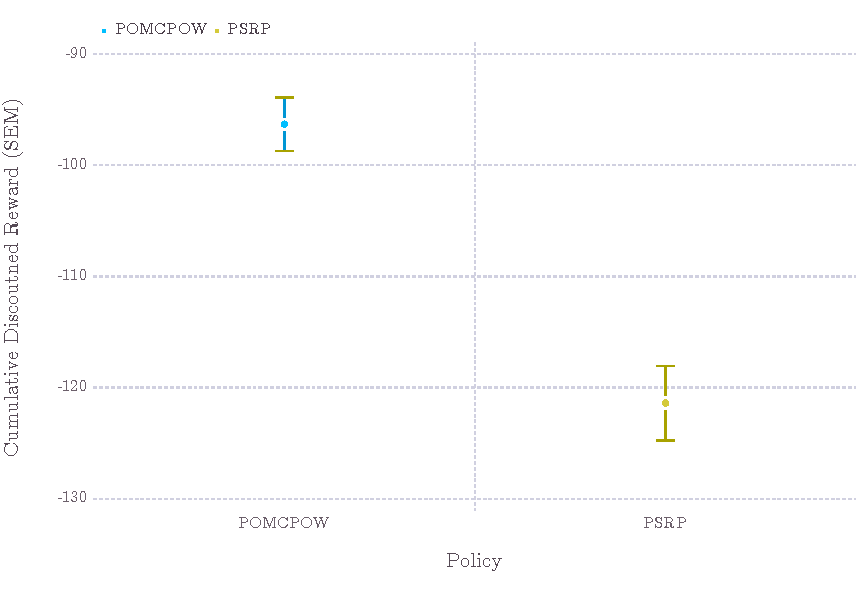
\includegraphics[scale=1]{hri_plots/hri_value_sem_plot.pdf}
  \caption{Mean and \acf{sem} of the cumulative discounted reward for
  \ac{pomcpow} (blue) and \ac{psrp} (yellow) as introduced in \cref{sec:hri-solutions}.}
  \label{fig:hri_eval_value_sem}
\end{figure}

Further insight is gained by evaluating the outcome statistics for each policy.
\Cref{fig:hri_outcome_histogram} depicts the frequencies of outcomes for each
policy. Since both policies reach a terminal state within the simulated horizon
for all sampled scenarios, here we only consider two classes of outcomes:
\emph{success}, the robot reached the goal location; and \emph{failure} the
robot collided with a wall or the human. The outcome statistics show that both
policies are able to successfully navigate the robot to its goal location in
the vast majority of all scenarios. However, \ac{pomcpow} still performs
significantly better with respect to safety. In fact, the collision rate in the
sampled scenarios for \ac{pomcpow} ($3.40\%$) is only half has high as for
\ac{psrp} ($7.08\%$).
% \todo[inline]{Should I note the adversarial character of these examples: many scenarios are rejected}

\begin{figure}[H]
  \centering
  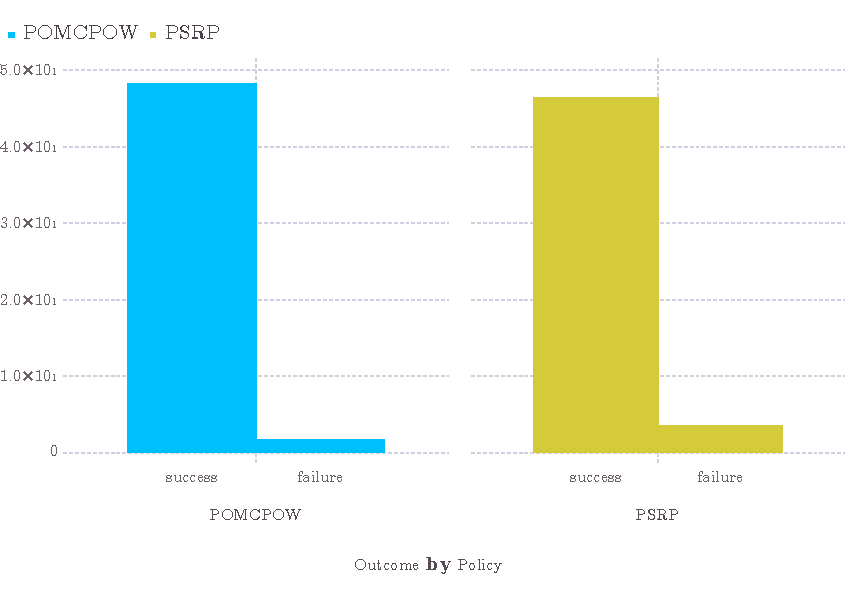
\includegraphics[scale=1]{hri_plots/hri_outcome_histogram_plot.pdf}
  \caption{Histogram of outcome frequencies grouped by policy. Outcome classes:
  \emph{success}, the robot reached the goal location; and \emph{failure} the
  robot collided with a wall or the human.}
  \label{fig:hri_outcome_histogram}
\end{figure}

While \ac{pomcpow} provides quantifiable better behaviors, this advantage comes
at the cost of higher computational effort. On average, decision making in
\ac{pomcpow} takes $\SI{0.279}{s}$ while for \ac{psrp} a decision is computed
within $\SI{0.042}{s}$.

A qualitative analysis of the behaviors generated by each solvers provides
further insight into the reasons for this gap in performance. We observe that
in many cases both solvers follow very similar strategies. When the human walks
towards one of the goal locations known by the robot, her decisions are well
explained by the behavior model used by the planner. In these cases, the model
confidence, $\beta$, increases and the planner is able to make confident
predictions of the future human position. Hence, for sufficiently high values
of $\beta$ the problem essentially approaches a deterministic planning problem.
Under these conditions \ac{psrp} performs equally well as \ac{pomcpow} since
optimal planning with probabilistic obstacles reliably finds suitable
trajectories to avoid collisions and reach the goal efficiently. In fact, in
the limit of $\beta \to \infty$ observation branching as employed by
\ac{pomcpow} is rendered obsolete.

Furthermore, in the problem discussed here the human does not react to the
robot. Therefore, observations whose statistics depend on latent variables are
independent of the robot action. As a result, in contrast to the application
domain discussed in \cref{chap:localization-and-planning} this problem does not
enable active information gathering. This property induced by the problem
structure further reduces the effect of observation branching.\\ However, there
still is a decisive difference between both strategies that causes the
performance gap observed above. In cases where the human appears to act
irrationally, the model confidence decreases and \cref{eq:boltzmann} essentially
becomes a uniform distribution. As as a result, the sequence of probabilistic
predictions used in \ac{psrp} features rapidly expanding uncertainty and the
planner has to avoid a large region of the state space. We observe that during
these maneuvers the agent often gets trapped in a corner of the room. When
using \ac{pomcpow} on the other hand, the agent is aware that it will get
further information to reduce the uncertainty in the future. Hence, the agent
is able to approach the human more confidently, enabling the robot to navigate
around the human in a less reactive manner.

In summary we can state that for the application example discussed in this
chapter the difference between the domain specific solver, \ac{psrp}, and the
generic \ac{pomdp} solver, \ac{pomcpow}, is less dramatic. Since by design the
problem does not allow for active information gathering, in many cases both
solvers generate similar behaviors. However, when faced with significant
uncertainty over the human intention, \ac{pomcpow} is still able to navigate
more safely, since observation branching allows to keep uncertainty over future
human positions bounded.

%  \begin{figure}[htpb]
%    \centering
%    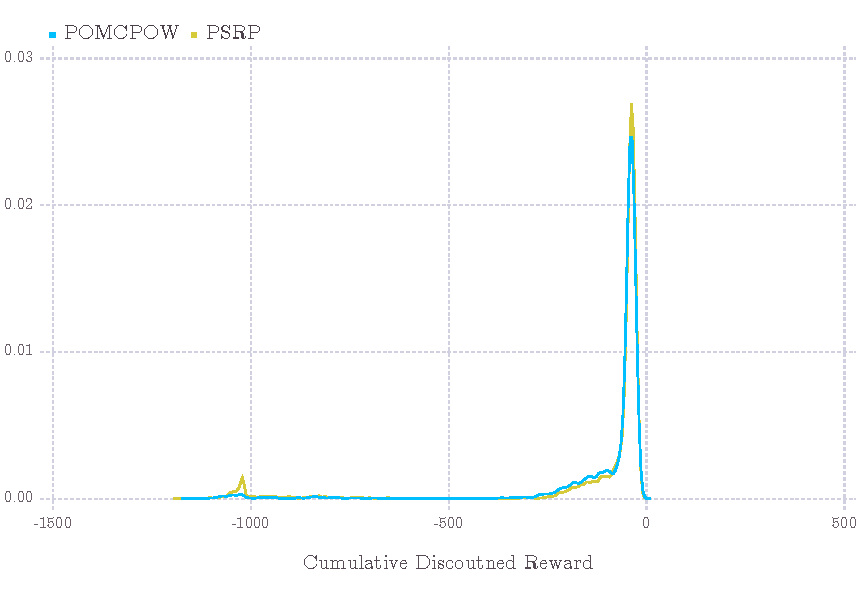
\includegraphics[scale=1]{hri_plots/hri_value_density_plot.pdf}
%    \caption{TODO}
%    \label{fig:hri_eval_value_density}
%  \end{figure}
%  
%  \begin{figure}[htpb]
%    \centering
%    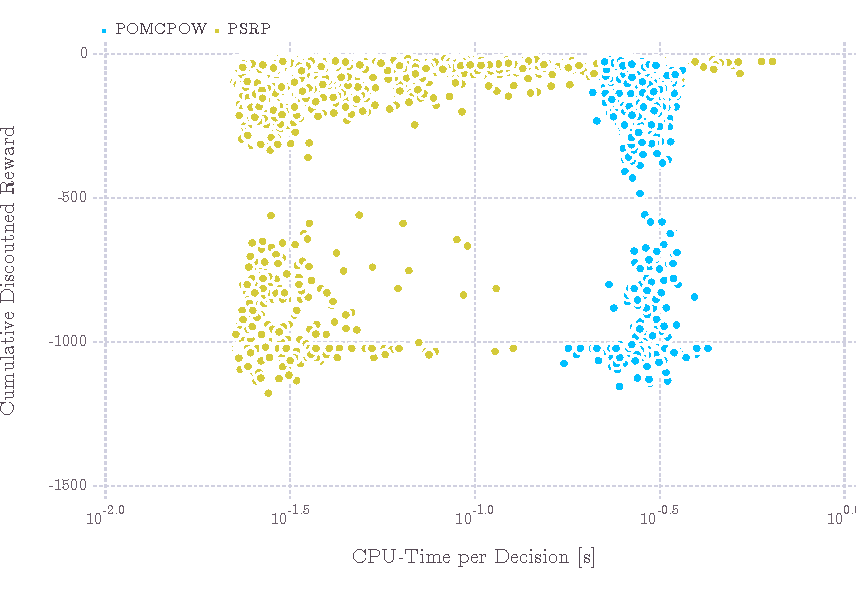
\includegraphics[scale=1]{hri_plots/hri_value_compute_scatter_plot.pdf}
%    \caption{TODO}
%    \label{fig:hri_eval_value_compute_scatter}
%  \end{figure}
%  
%  \begin{figure}[htpb]
%    \centering
%    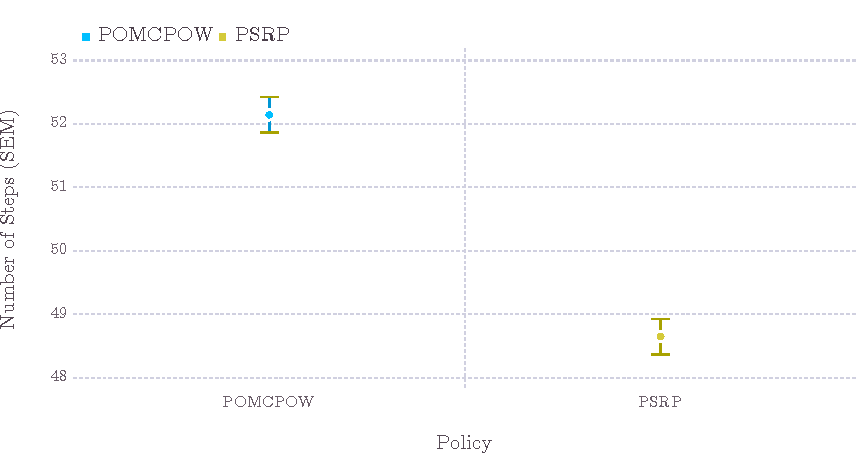
\includegraphics[scale=1]{hri_plots/hri_nstep_sem_plot.pdf}
%    \caption{TODO}
%    \label{fig:hri_eval_nstep_sem}
%  \end{figure}
%  
%  \begin{figure}[htpb]
%    \centering
%    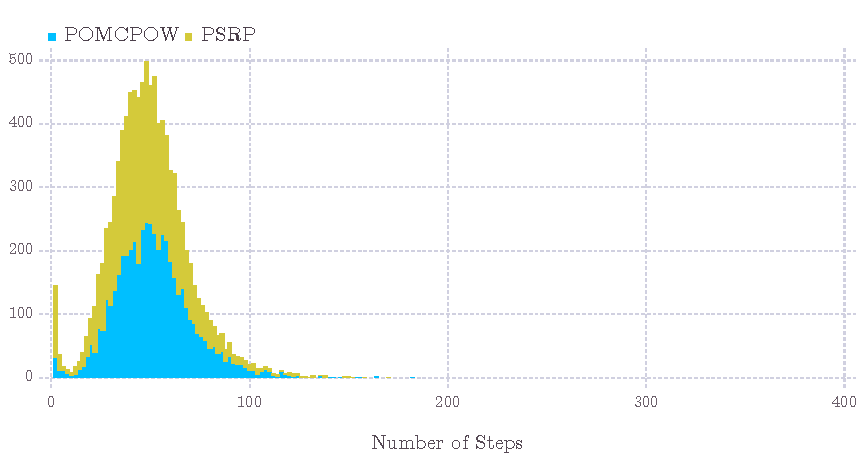
\includegraphics[scale=1]{hri_plots/hri_nstep_density_plot.pdf}
%    \caption{TODO}
%    \label{fig:hri_eval_nstep_density}
%  \end{figure}
%  
%  \begin{figure}[htpb]
%    \centering
%    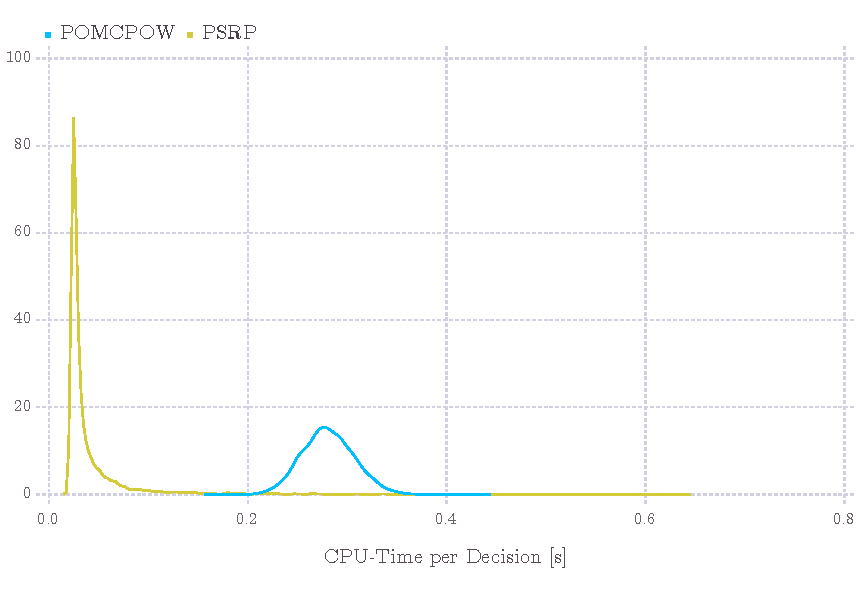
\includegraphics[scale=1]{hri_plots/hri_compute_density_plot.pdf}
%    \caption{TODO}
%    \label{fig:hri_eval_compute_density}
%  \end{figure}

\iffalse
\chapter{Discussion}\label{chap:discussion}

\todo[inline]{Note: The analysis/discussion for each application example has
been "inlined" with the qualitative analysis at the end of each chapter. In
this chapter I now only summarize the mechanisms and give some advice for "when
does it make sense to model a problem as a POMDP". Maybe this is not enough for
a whole chapter and rather redundant.}

The experiments presented in \cref{chap:localization-and-planning,chap:hri}
show that \ac{pomdp} solvers are able to generate well performing behaviors for
different planning problems. The quantitative and qualitative analysis
performed for these examples reveal that the benefits provided by this kind of
reasoning are cause by different mechanisms.

\begin{itemize}
  \item prob obstacles is technically a nice idea but it only works for this very problem structure
  \item this kind of reasoning does not work when the human reacts to the robot since open loop predictions
  require knowledge of the robot position in the future.
\end{itemize}

\todo[inline]{This section will mainly contain the "lessons learned"
+ a comparison between the problems, explaining the mechanisms which lead to
the improvement in each case.}

\begin{itemize}
  \item \acp{pomdp} provide an elegant way of closing the loop between
    prediction (and perception models) and planning.
  \item This provides benefits through various mechanisms:
  \item Simultaneous localization and planning: Using a \ac{pomdp} leads to active
    information gathering and provides a principled, optimization based
    approach to solving this problem (even under massive uncertainty). Solving
    it without such procedure is not straightforward, since planning on expectation
    with these highly multi-modal belief topologies is impractical.
  \item Planning with latent human intentions: The \ac{pomdp} based solution
    allows the robot to consider future observations, making the robots plans
    less conservative because the agent knows that uncertainty about the humans intentions
    will be reduced in the future. For this very problem structure, neglecting future observations
    provides a principled way of solving this problem. Through this
    approximation, the problem is simplified to a problem that is still
    NP-hard, but well studied. Good heuristics exist, such that search is well guided to find results
    withing reasonable planning horizons. However, sacrificing performance (in
    particular for models with unbounded uncertainty like constant velocity).
    \begin{itemize}
      \item Future work: \ac{pomdp} solution method is safer than planning with
      probabilistic obstacles while reaching the goal in fewer number of steps.
      However, probabilistic obstacles can provide a-priory estimate of safety
      while for \acp{pomdp} this can only be shown empirically through large
      scale simulations. It would be nice to provide a safety assurance for
      this special type of \acp{pomdp} (Mixed Observability Markov Decision
      Process where the safety only depends on some unactuated decoupled part
      of the state.)
    \end{itemize}
\end{itemize}
\fi

\chapter{Summary}

\chapter{Formatting - TODO}

\begin{itemize}
  \item genitive "s" (robots vs. robot's, its vs it's)
  \item Introduction must be page one (see TOC)
  \item (done) ix acronym capitalization
  \item maybe have acronyms rendered in italic
  \item section references in caps?
  \item look for common spelling mistakes
  \item look for "will", most things should be "present"
  \item avoid "don't", "won't", "doesn't" etc.\
  \item flows $\to$ follows
\end{itemize}


% add bibliography to table of contents
\ifthenelse{\equal{1}{0}}
    {\bibliographystyle{mum_deu} % deutsches Lit.verzeichnis
    }{}
\ifthenelse{\equal{1}{1}}
    {\bibliographystyle{mum_en} % englisches Lit.verzeichnis z.B. statt "S." nun "p." bzw. "pp."
    }{}

\phantomsection

\ifthenelse{\equal{1}{0}}
    {\addcontentsline{toc}{chapter}{Literaturverzeichnis}
    }{}
\ifthenelse{\equal{1}{1}}
    {\addcontentsline{toc}{chapter}{Bibliography}
    }{}
\bibliography{lit/thesis.bib}
%###########################################################################
%
%   Anhang
%
%###########################################################################
\begin{appendix}
\ifthenelse{\equal{\Sprache}{0}}
{\chapter*{Anhang}\label{sec:Anhang}
	\setcounter{chapter}{1}
	\addcontentsline{toc}{chapter}{Anhang}
}{}
\ifthenelse{\equal{\Sprache}{1}}
{\chapter*{Appendix}\label{sec:appendix}
	\setcounter{chapter}{1}
	\addcontentsline{toc}{chapter}{Appendix}
}{}


%###########################################################################
%   Anhang A
%###########################################################################
\ifthenelse{\equal{\Sprache}{0}}
{\section{Inhalt Archiv}\label{sec:AnhangArchiv}
	\markboth{Anhang}{Anhang}
	%
	%
	Im Archiv ist ein Verzeichnis
\RemoveSpaces{
	\ifthenelse{\equal{\MScBSc}{0}}
	{\textbf{BSC$\_$\NummerDerArbeit$\_$\NachnameDesStudenten/}}{}
	\ifthenelse{\equal{\MScBSc}{1}}
	{\textbf{PRO$\_$\NummerDerArbeit$\_$\NachnameDesStudenten/}}{}
	\ifthenelse{\equal{\MScBSc}{2}}
	{\textbf{MSC$\_$\NummerDerArbeit$\_$\NachnameDesStudenten/}}{}
} abgelegt.
Dieses enthält in der obersten Dateistruktur die Einträge
	\begin{itemize}
	\item \ifthenelse{\equal{\MScBSc}{0}}
		{\textbf{BSC$\_$\NummerDerArbeit$\_$\NachnameDesStudenten.pdf}:}{}
		\ifthenelse{\equal{\MScBSc}{1}}
		{\textbf{PRO$\_$\NummerDerArbeit$\_$\NachnameDesStudenten.pdf}:}{}
		\ifthenelse{\equal{\MScBSc}{2}}
		{\textbf{MSC$\_$\NummerDerArbeit$\_$\NachnameDesStudenten.pdf}:}{}
		das pdf-File zur Arbeit
\RemoveSpaces{
		\ifthenelse{\equal{\MScBSc}{0}}
		{BSC-\NummerDerArbeit.}{}
		\ifthenelse{\equal{\MScBSc}{1}}
		{PRO-\NummerDerArbeit.}{}
		\ifthenelse{\equal{\MScBSc}{2}}
		{MSC-\NummerDerArbeit.}{}
}
		%
		\item \textbf{Daten/}: ein Verzeichnis mit den für diese Arbeit
		relevanten Daten, Hilfsprogrammen, Skripts und Simulationsumgebungen.
		\item \textbf{Latex/}: ein Verzeichnis mit den *.tex-Dateien des in
		Latex verfassten Berichts zur Arbeit
\RemoveSpaces{
		\ifthenelse{\equal{\MScBSc}{0}}
		{BSC-\NummerDerArbeit}{}
		\ifthenelse{\equal{\MScBSc}{1}}
		{PRO-\NummerDerArbeit}{}
		\ifthenelse{\equal{\MScBSc}{2}}
		{MSC-\NummerDerArbeit}{}
}
		sowie alle dazugehörigen Grafiken (falls vorhanden auch als *.svg Dateien).
		%
		\item \textbf{Vortrag/}: ein Verzeichnis mit den für den Vortrag relevanten Daten wie die Präsentation, Bilder und Videos.
		%
	\end{itemize}
}{}
\ifthenelse{\equal{\Sprache}{1}}
{\section{Contents Archive}\label{apx:archive}
	\markboth{Appendix}{Appendix}
	%
	%
	There is a folder
\RemoveSpaces{
	\ifthenelse{\equal{\MScBSc}{0}}
	{\textbf{BSC$\_$\NummerDerArbeit$\_$\NachnameDesStudenten/}}{}
	\ifthenelse{\equal{\MScBSc}{1}}
	{\textbf{PRO$\_$\NummerDerArbeit$\_$\NachnameDesStudenten/}}{}
	\ifthenelse{\equal{\MScBSc}{2}}
	{\textbf{MSC$\_$\NummerDerArbeit$\_$\NachnameDesStudenten/}}{}} in the archive. The main folder contains the entries
	\begin{itemize}
		\item \ifthenelse{\equal{\MScBSc}{0}}
		{\textbf{BSC$\_$\NummerDerArbeit$\_$\NachnameDesStudenten.pdf}:}{}
		\ifthenelse{\equal{\MScBSc}{1}}
		{\textbf{PRO$\_$\NummerDerArbeit$\_$\NachnameDesStudenten.pdf}:}{}
		\ifthenelse{\equal{\MScBSc}{2}}
		{\textbf{MSC$\_$\NummerDerArbeit$\_$\NachnameDesStudenten.pdf}:}{}
		the pdf-file of the thesis
\RemoveSpaces{
		\ifthenelse{\equal{\MScBSc}{0}}
		{BSC-\NummerDerArbeit.}{}
		\ifthenelse{\equal{\MScBSc}{1}}
		{PRO-\NummerDerArbeit.}{}
		\ifthenelse{\equal{\MScBSc}{2}}
		{MSC-\NummerDerArbeit.}{}}
		%
		\item \textbf{Data/}: a folder with all the relevant data, programs, scripts and simulation environments.
		\item \textbf{Latex/}: a folder with the *.tex documents of the thesis
\RemoveSpaces{
		\ifthenelse{\equal{\MScBSc}{0}}
		{BSC-\NummerDerArbeit}{}
		\ifthenelse{\equal{\MScBSc}{1}}
		{PRO-\NummerDerArbeit}{}
		\ifthenelse{\equal{\MScBSc}{2}}
		{MSC-\NummerDerArbeit}{}}
		written in Latex and all figures (also in *.svg data format if available).
		%
		\item \textbf{Presentation/}: a folder with the relevant data for the presentation including the presentation itself, figures and videos.
		%
	\end{itemize}
}{}

\section{Comparison of \ac{mlra} and \ac{mlmpc} for the Fully Observable Case}\label{apx:fo-comparison}

\missingfigure{mlra vs mlmpc}

%###########################################################################
\end{appendix}

\thispagestyle{empty}\cleardoublepage
%Selbstständigkeitserklärung

\thispagestyle{plain}
\large
\selectlanguage{ngerman}
%\begin{flushright}
%  Hamburg, den \today
%\end{flushright}
\textbf{Erklärung}
\vspace*{5mm}

Ich, {\VornameDesStudenten \ \NachnameDesStudenten} (\Studiengang~an der Technischen 
Universität Hamburg-Harburg, Matrikelnummer \Matrikelnummer), versichere, dass ich die vorliegende 
\RemoveSpaces{		
		{\ifthenelse{\equal{\MScBSc}{0}}
			{Bachelorarbeit}{}
		\ifthenelse{\equal{\MScBSc}{1}}
			{Projektarbeit}{}
		\ifthenelse{\equal{\MScBSc}{2}}
			{Masterarbeit}{}}}
selbstständig verfasst und keine anderen als die angegebenen Hilfsmittel verwendet habe. Die Arbeit wurde in dieser oder ähnlicher Form noch keiner Prüfungskommission vorgelegt.\\

\vspace*{50mm}

\begin{center}
\noindent\begin{tabular}{c}
\makebox[\widthof{\VornameDesStudenten\NachnameDesStudenten}+1in]{\hrulefill}\\
{ Unterschrift} \\[8ex]% adds space between the two sets of signatures
\end{tabular}
\noindent\begin{tabular}{c}
\makebox[1.75in]{\hrulefill}\\
Datum\\[8ex]
\end{tabular}
\end{center}
  


\normalsize

\end{document}
